\documentclass[1p]{elsarticle_modified}
%\bibliographystyle{elsarticle-num}

%\usepackage[colorlinks]{hyperref}
%\usepackage{abbrmath_seonhwa} %\Abb, \Ascr, \Acal ,\Abf, \Afrak
\usepackage{amsfonts}
\usepackage{amssymb}
\usepackage{amsmath}
\usepackage{amsthm}
\usepackage{scalefnt}
\usepackage{amsbsy}
\usepackage{kotex}
\usepackage{caption}
\usepackage{subfig}
\usepackage{color}
\usepackage{graphicx}
\usepackage{xcolor} %% white, black, red, green, blue, cyan, magenta, yellow
\usepackage{float}
\usepackage{setspace}
\usepackage{hyperref}

\usepackage{tikz}
\usetikzlibrary{arrows}

\usepackage{multirow}
\usepackage{array} % fixed length table
\usepackage{hhline}

%%%%%%%%%%%%%%%%%%%%%
\makeatletter
\renewcommand*\env@matrix[1][\arraystretch]{%
	\edef\arraystretch{#1}%
	\hskip -\arraycolsep
	\let\@ifnextchar\new@ifnextchar
	\array{*\c@MaxMatrixCols c}}
\makeatother %https://tex.stackexchange.com/questions/14071/how-can-i-increase-the-line-spacing-in-a-matrix
%%%%%%%%%%%%%%%

\usepackage[normalem]{ulem}

\newcommand{\msout}[1]{\ifmmode\text{\sout{\ensuremath{#1}}}\else\sout{#1}\fi}
%SOURCE: \msout is \stkout macro in https://tex.stackexchange.com/questions/20609/strikeout-in-math-mode

\newcommand{\cancel}[1]{
	\ifmmode
	{\color{red}\msout{#1}}
	\else
	{\color{red}\sout{#1}}
	\fi
}

\newcommand{\add}[1]{
	{\color{blue}\uwave{#1}}
}

\newcommand{\replace}[2]{
	\ifmmode
	{\color{red}\msout{#1}}{\color{blue}\uwave{#2}}
	\else
	{\color{red}\sout{#1}}{\color{blue}\uwave{#2}}
	\fi
}

\newcommand{\Sol}{\mathcal{S}} %segment
\newcommand{\D}{D} %diagram
\newcommand{\A}{\mathcal{A}} %arc


%%%%%%%%%%%%%%%%%%%%%%%%%%%%%5 test

\def\sl{\operatorname{\textup{SL}}(2,\Cbb)}
\def\psl{\operatorname{\textup{PSL}}(2,\Cbb)}
\def\quan{\mkern 1mu \triangleright \mkern 1mu}

\theoremstyle{definition}
\newtheorem{thm}{Theorem}[section]
\newtheorem{prop}[thm]{Proposition}
\newtheorem{lem}[thm]{Lemma}
\newtheorem{ques}[thm]{Question}
\newtheorem{cor}[thm]{Corollary}
\newtheorem{defn}[thm]{Definition}
\newtheorem{exam}[thm]{Example}
\newtheorem{rmk}[thm]{Remark}
\newtheorem{alg}[thm]{Algorithm}

\newcommand{\I}{\sqrt{-1}}
\begin{document}

%\begin{frontmatter}
%
%\title{Boundary parabolic representations of knots up to 8 crossings}
%
%%% Group authors per affiliation:
%\author{Yunhi Cho} 
%\address{Department of Mathematics, University of Seoul, Seoul, Korea}
%\ead{yhcho@uos.ac.kr}
%
%
%\author{Seonhwa Kim} %\fnref{s_kim}}
%\address{Center for Geometry and Physics, Institute for Basic Science, Pohang, 37673, Korea}
%\ead{ryeona17@ibs.re.kr}
%
%\author{Hyuk Kim}
%\address{Department of Mathematical Sciences, Seoul National University, Seoul 08826, Korea}
%\ead{hyukkim@snu.ac.kr}
%
%\author{Seokbeom Yoon}
%\address{Department of Mathematical Sciences, Seoul National University, Seoul, 08826,  Korea}
%\ead{sbyoon15@snu.ac.kr}
%
%\begin{abstract}
%We find all boundary parabolic representation of knots up to 8 crossings.
%
%\end{abstract}
%\begin{keyword}
%    \MSC[2010] 57M25 
%\end{keyword}
%
%\end{frontmatter}

%\linenumbers
%\tableofcontents
%
\newcommand\colored[1]{\textcolor{white}{\rule[-0.35ex]{0.8em}{1.4ex}}\kern-0.8em\color{red} #1}%
%\newcommand\colored[1]{\textcolor{white}{ #1}\kern-2.17ex	\textcolor{white}{ #1}\kern-1.81ex	\textcolor{white}{ #1}\kern-2.15ex\color{red}#1	}

{\Large $\underline{12a_{0044}~(K12a_{0044})}$}

\setlength{\tabcolsep}{10pt}
\renewcommand{\arraystretch}{1.6}
\vspace{1cm}\begin{tabular}{m{100pt}>{\centering\arraybackslash}m{274pt}}
\multirow{5}{120pt}{
	\centering
	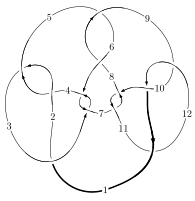
\includegraphics[width=112pt]{../../../GIT/diagram.site/Diagrams/png/845_12a_0044.png}\\
\ \ \ A knot diagram\footnotemark}&
\allowdisplaybreaks
\textbf{Linearized knot diagam} \\
\cline{2-2}
 &
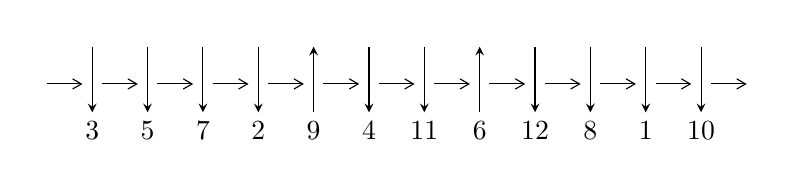
\begin{tikzpicture}[x=20pt, y=17pt]
	% nodes
	\node (C0) at (0, 0) {};
	\node (C1) at (1, 0) {};
	\node (C1U) at (1, +1) {};
	\node (C1D) at (1, -1) {3};

	\node (C2) at (2, 0) {};
	\node (C2U) at (2, +1) {};
	\node (C2D) at (2, -1) {5};

	\node (C3) at (3, 0) {};
	\node (C3U) at (3, +1) {};
	\node (C3D) at (3, -1) {7};

	\node (C4) at (4, 0) {};
	\node (C4U) at (4, +1) {};
	\node (C4D) at (4, -1) {2};

	\node (C5) at (5, 0) {};
	\node (C5U) at (5, +1) {};
	\node (C5D) at (5, -1) {9};

	\node (C6) at (6, 0) {};
	\node (C6U) at (6, +1) {};
	\node (C6D) at (6, -1) {4};

	\node (C7) at (7, 0) {};
	\node (C7U) at (7, +1) {};
	\node (C7D) at (7, -1) {11};

	\node (C8) at (8, 0) {};
	\node (C8U) at (8, +1) {};
	\node (C8D) at (8, -1) {6};

	\node (C9) at (9, 0) {};
	\node (C9U) at (9, +1) {};
	\node (C9D) at (9, -1) {12};

	\node (C10) at (10, 0) {};
	\node (C10U) at (10, +1) {};
	\node (C10D) at (10, -1) {8};

	\node (C11) at (11, 0) {};
	\node (C11U) at (11, +1) {};
	\node (C11D) at (11, -1) {1};

	\node (C12) at (12, 0) {};
	\node (C12U) at (12, +1) {};
	\node (C12D) at (12, -1) {10};
	\node (C13) at (13, 0) {};

	% arrows
	\draw[->,>={angle 60}]
	(C0) edge (C1) (C1) edge (C2) (C2) edge (C3) (C3) edge (C4) (C4) edge (C5) (C5) edge (C6) (C6) edge (C7) (C7) edge (C8) (C8) edge (C9) (C9) edge (C10) (C10) edge (C11) (C11) edge (C12) (C12) edge (C13) ;	\draw[->,>=stealth]
	(C1U) edge (C1D) (C2U) edge (C2D) (C3U) edge (C3D) (C4U) edge (C4D) (C5D) edge (C5U) (C6U) edge (C6D) (C7U) edge (C7D) (C8D) edge (C8U) (C9U) edge (C9D) (C10U) edge (C10D) (C11U) edge (C11D) (C12U) edge (C12D) ;
	\end{tikzpicture} \\
\hhline{~~} \\& 
\textbf{Solving Sequence} \\ \cline{2-2} 
 &
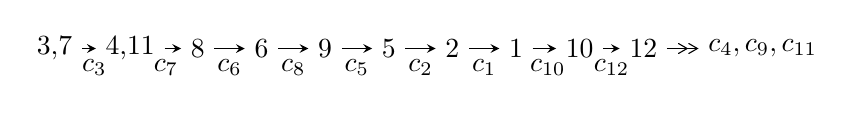
\begin{tikzpicture}[x=23pt, y=7pt]
	% node
	\node (A0) at (-1/8, 0) {3,7};
	\node (A1) at (17/16, 0) {4,11};
	\node (A2) at (17/8, 0) {8};
	\node (A3) at (25/8, 0) {6};
	\node (A4) at (33/8, 0) {9};
	\node (A5) at (41/8, 0) {5};
	\node (A6) at (49/8, 0) {2};
	\node (A7) at (57/8, 0) {1};
	\node (A8) at (65/8, 0) {10};
	\node (A9) at (73/8, 0) {12};
	\node (C1) at (1/2, -1) {$c_{3}$};
	\node (C2) at (13/8, -1) {$c_{7}$};
	\node (C3) at (21/8, -1) {$c_{6}$};
	\node (C4) at (29/8, -1) {$c_{8}$};
	\node (C5) at (37/8, -1) {$c_{5}$};
	\node (C6) at (45/8, -1) {$c_{2}$};
	\node (C7) at (53/8, -1) {$c_{1}$};
	\node (C8) at (61/8, -1) {$c_{10}$};
	\node (C9) at (69/8, -1) {$c_{12}$};
	\node (A10) at (11, 0) {$c_{4},c_{9},c_{11}$};

	% edge
	\draw[->,>=stealth]	
	(A0) edge (A1) (A1) edge (A2) (A2) edge (A3) (A3) edge (A4) (A4) edge (A5) (A5) edge (A6) (A6) edge (A7) (A7) edge (A8) (A8) edge (A9) ;
	\draw[->>,>={angle 60}]	
	(A9) edge (A10);
\end{tikzpicture} \\ 

\end{tabular} \\

\footnotetext{
The image of knot diagram is generated by the software ``\textbf{Draw programme}" developed by Andrew Bartholomew(\url{http://www.layer8.co.uk/maths/draw/index.htm\#Running-draw}), where we modified some parts for our purpose(\url{https://github.com/CATsTAILs/LinksPainter}).
}\phantom \\ \newline 
\centering \textbf{Ideals for irreducible components\footnotemark of $X_{\text{par}}$} 
 
\begin{align*}
I^u_{1}&=\langle 
-84627704 u^{20}-128973875 u^{19}+\cdots+51452411 b-272407188,\;a-1,\;u^{21}+u^{20}+\cdots+4 u-1\rangle \\
I^u_{2}&=\langle 
5.22206\times10^{409} u^{113}+1.42485\times10^{410} u^{112}+\cdots+5.53920\times10^{411} b+3.35281\times10^{412},\\
\phantom{I^u_{2}}&\phantom{= \langle  }-1.67844\times10^{410} u^{113}-6.46598\times10^{410} u^{112}+\cdots+1.10784\times10^{412} a+1.29452\times10^{413},\\
\phantom{I^u_{2}}&\phantom{= \langle  }u^{114}+4 u^{113}+\cdots-9216 u-512\rangle \\
I^u_{3}&=\langle 
- u^8-2 u^7-4 u^6-4 u^5-6 u^4-5 u^3-6 u^2+b-3 u-3,\;a,\;u^9+u^8+2 u^7+u^6+3 u^5+u^4+2 u^3+u-1\rangle \\
I^u_{4}&=\langle 
u^2+b+2,\;a+1,\;u^3- u^2+2 u-1\rangle \\
I^u_{5}&=\langle 
-2 a u+b+2 u-1,\;u^2 a+a^2- a u+3 u^2+a- u+5,\;u^3- u^2+2 u-1\rangle \\
\\
I^v_{1}&=\langle 
a,\;4 v^8-372 v^7-2334 v^6-5550 v^5-4357 v^4+2618 v^3+3887 v^2+683 b-3400 v-4863,\\
\phantom{I^v_{1}}&\phantom{= \langle  }v^9+7 v^8+20 v^7+25 v^6+5 v^5-15 v^4+22 v^2+13 v-1\rangle \\
\end{align*}
\raggedright * 6 irreducible components of $\dim_{\mathbb{C}}=0$, with total 162 representations.\\
\footnotetext{All coefficients of polynomials are rational numbers. But the coefficients are sometimes approximated in decimal forms when there is not enough margin.}
\newpage
\renewcommand{\arraystretch}{1}
\centering \section*{I. $I^u_{1}= \langle -8.46\times10^{7} u^{20}-1.29\times10^{8} u^{19}+\cdots+5.15\times10^{7} b-2.72\times10^{8},\;a-1,\;u^{21}+u^{20}+\cdots+4 u-1 \rangle$}
\flushleft \textbf{(i) Arc colorings}\\
\begin{tabular}{m{7pt} m{180pt} m{7pt} m{180pt} }
\flushright $a_{3}=$&$\begin{pmatrix}1\\0\end{pmatrix}$ \\
\flushright $a_{7}=$&$\begin{pmatrix}0\\u\end{pmatrix}$ \\
\flushright $a_{4}=$&$\begin{pmatrix}1\\u^2\end{pmatrix}$ \\
\flushright $a_{11}=$&$\begin{pmatrix}1\\1.64478 u^{20}+2.50666 u^{19}+\cdots-5.18329 u+5.29435\end{pmatrix}$ \\
\flushright $a_{8}=$&$\begin{pmatrix}- u\\-0.861887 u^{20}-0.812044 u^{19}+\cdots+2.28475 u-1.64478\end{pmatrix}$ \\
\flushright $a_{6}=$&$\begin{pmatrix}u\\u^3+u\end{pmatrix}$ \\
\flushright $a_{9}=$&$\begin{pmatrix}0.192548 u^{20}-0.0736292 u^{19}+\cdots-2.06126 u+0.0498433\\-0.603909 u^{20}-0.670769 u^{19}+\cdots+2.48075 u-1.86111\end{pmatrix}$ \\
\flushright $a_{5}=$&$\begin{pmatrix}-0.265940 u^{20}+0.118547 u^{19}+\cdots+2.50924 u-0.0261450\\0.310547 u^{20}+0.573803 u^{19}+\cdots-1.29066 u+1.04156\end{pmatrix}$ \\
\flushright $a_{2}=$&$\begin{pmatrix}-0.265940 u^{20}+0.118547 u^{19}+\cdots+2.50924 u-0.0261450\\-0.276831 u^{20}-0.685016 u^{19}+\cdots-0.513226 u-0.657077\end{pmatrix}$ \\
\flushright $a_{1}=$&$\begin{pmatrix}-0.542770 u^{20}-0.566469 u^{19}+\cdots+1.99601 u-0.683222\\-0.276831 u^{20}-0.685016 u^{19}+\cdots-0.513226 u-0.657077\end{pmatrix}$ \\
\flushright $a_{10}=$&$\begin{pmatrix}u^2+1\\1.59493 u^{20}+2.26427 u^{19}+\cdots-6.98606 u+6.15624\end{pmatrix}$ \\
\flushright $a_{12}=$&$\begin{pmatrix}-0.293060 u^{20}-0.196829 u^{19}+\cdots-0.0371231 u+0.621597\\1.30711 u^{20}+1.61748 u^{19}+\cdots-6.43899 u+4.90053\end{pmatrix}$\\&\end{tabular}
\flushleft \textbf{(ii) Obstruction class $= -1$}\\~\\
\flushleft \textbf{(iii) Cusp Shapes $= -\frac{1476285438}{51452411} u^{20}-\frac{1893823898}{51452411} u^{19}+\cdots+\frac{5145089090}{51452411} u-\frac{4384281402}{51452411}$}\\~\\
\newpage\renewcommand{\arraystretch}{1}
\flushleft \textbf{(iv) u-Polynomials at the component}\newline \\
\begin{tabular}{m{50pt}|m{274pt}}
Crossings & \hspace{64pt}u-Polynomials at each crossing \\
\hline $$\begin{aligned}c_{1},c_{11}\end{aligned}$$&$\begin{aligned}
&u^{21}+11 u^{20}+\cdots-4 u+1
\end{aligned}$\\
\hline $$\begin{aligned}c_{2},c_{4},c_{9}\\c_{12}\end{aligned}$$&$\begin{aligned}
&u^{21}-3 u^{20}+\cdots-2 u+1
\end{aligned}$\\
\hline $$\begin{aligned}c_{3},c_{6},c_{7}\\c_{10}\end{aligned}$$&$\begin{aligned}
&u^{21}- u^{20}+\cdots+4 u+1
\end{aligned}$\\
\hline $$\begin{aligned}c_{5},c_{8}\end{aligned}$$&$\begin{aligned}
&u^{21}+7 u^{20}+\cdots-24 u-8
\end{aligned}$\\
\hline
\end{tabular}\\~\\
\newpage\renewcommand{\arraystretch}{1}
\flushleft \textbf{(v) Riley Polynomials at the component}\newline \\
\begin{tabular}{m{50pt}|m{274pt}}
Crossings & \hspace{64pt}Riley Polynomials at each crossing \\
\hline $$\begin{aligned}c_{1},c_{11}\end{aligned}$$&$\begin{aligned}
&y^{21}+y^{20}+\cdots+60 y-1
\end{aligned}$\\
\hline $$\begin{aligned}c_{2},c_{4},c_{9}\\c_{12}\end{aligned}$$&$\begin{aligned}
&y^{21}-11 y^{20}+\cdots-4 y-1
\end{aligned}$\\
\hline $$\begin{aligned}c_{3},c_{6},c_{7}\\c_{10}\end{aligned}$$&$\begin{aligned}
&y^{21}+9 y^{20}+\cdots+4 y-1
\end{aligned}$\\
\hline $$\begin{aligned}c_{5},c_{8}\end{aligned}$$&$\begin{aligned}
&y^{21}+7 y^{20}+\cdots+384 y-64
\end{aligned}$\\
\hline
\end{tabular}\\~\\
\newpage\flushleft \textbf{(vi) Complex Volumes and Cusp Shapes}
$$\begin{array}{c|c|c}  
\text{Solutions to }I^u_{1}& \I (\text{vol} + \sqrt{-1}CS) & \text{Cusp shape}\\
 \hline 
\begin{aligned}
u &= -0.654628 + 0.778929 I \\
a &= \phantom{-}1.00000\phantom{ +0.000000I} \\
b &= \phantom{-}0.301139 - 1.121240 I\end{aligned}
 & -6.57363 + 8.18913 I & -13.0291 - 11.3346 I \\ \hline\begin{aligned}
u &= -0.654628 - 0.778929 I \\
a &= \phantom{-}1.00000\phantom{ +0.000000I} \\
b &= \phantom{-}0.301139 + 1.121240 I\end{aligned}
 & -6.57363 - 8.18913 I & -13.0291 + 11.3346 I \\ \hline\begin{aligned}
u &= -0.448527 + 0.840581 I \\
a &= \phantom{-}1.00000\phantom{ +0.000000I} \\
b &= \phantom{-}2.61918 - 0.41086 I\end{aligned}
 & -5.92018 + 0.83164 I & -11.63192 - 4.49260 I \\ \hline\begin{aligned}
u &= -0.448527 - 0.840581 I \\
a &= \phantom{-}1.00000\phantom{ +0.000000I} \\
b &= \phantom{-}2.61918 + 0.41086 I\end{aligned}
 & -5.92018 - 0.83164 I & -11.63192 + 4.49260 I \\ \hline\begin{aligned}
u &= -1.041870 + 0.475093 I \\
a &= \phantom{-}1.00000\phantom{ +0.000000I} \\
b &= \phantom{-}1.97284 - 0.75695 I\end{aligned}
 & -4.35380 - 5.94110 I & -11.79339 + 6.03278 I \\ \hline\begin{aligned}
u &= -1.041870 - 0.475093 I \\
a &= \phantom{-}1.00000\phantom{ +0.000000I} \\
b &= \phantom{-}1.97284 + 0.75695 I\end{aligned}
 & -4.35380 + 5.94110 I & -11.79339 - 6.03278 I \\ \hline\begin{aligned}
u &= \phantom{-}0.752000 + 0.272051 I \\
a &= \phantom{-}1.00000\phantom{ +0.000000I} \\
b &= \phantom{-}2.06444 + 1.49682 I\end{aligned}
 & -2.27847 + 1.35735 I & -12.26664 - 3.16411 I \\ \hline\begin{aligned}
u &= \phantom{-}0.752000 - 0.272051 I \\
a &= \phantom{-}1.00000\phantom{ +0.000000I} \\
b &= \phantom{-}2.06444 - 1.49682 I\end{aligned}
 & -2.27847 - 1.35735 I & -12.26664 + 3.16411 I \\ \hline\begin{aligned}
u &= \phantom{-}0.148758 + 0.737388 I \\
a &= \phantom{-}1.00000\phantom{ +0.000000I} \\
b &= -0.679107 + 0.183414 I\end{aligned}
 & \phantom{-}0.94396 - 2.98921 I & -0.51194 + 9.40250 I \\ \hline\begin{aligned}
u &= \phantom{-}0.148758 - 0.737388 I \\
a &= \phantom{-}1.00000\phantom{ +0.000000I} \\
b &= -0.679107 - 0.183414 I\end{aligned}
 & \phantom{-}0.94396 + 2.98921 I & -0.51194 - 9.40250 I\\
 \hline 
 \end{array}$$\newpage$$\begin{array}{c|c|c}  
\text{Solutions to }I^u_{1}& \I (\text{vol} + \sqrt{-1}CS) & \text{Cusp shape}\\
 \hline 
\begin{aligned}
u &= -0.371460 + 1.226140 I \\
a &= \phantom{-}1.00000\phantom{ +0.000000I} \\
b &= \phantom{-}0.88921 - 1.56579 I\end{aligned}
 & \phantom{-}6.79620 + 1.15294 I & -1.115456 + 0.635021 I \\ \hline\begin{aligned}
u &= -0.371460 - 1.226140 I \\
a &= \phantom{-}1.00000\phantom{ +0.000000I} \\
b &= \phantom{-}0.88921 + 1.56579 I\end{aligned}
 & \phantom{-}6.79620 - 1.15294 I & -1.115456 - 0.635021 I \\ \hline\begin{aligned}
u &= \phantom{-}0.507858 + 0.499877 I \\
a &= \phantom{-}1.00000\phantom{ +0.000000I} \\
b &= \phantom{-}0.321354 + 0.105246 I\end{aligned}
 & -0.56389 - 1.48786 I & -4.78639 + 4.72577 I \\ \hline\begin{aligned}
u &= \phantom{-}0.507858 - 0.499877 I \\
a &= \phantom{-}1.00000\phantom{ +0.000000I} \\
b &= \phantom{-}0.321354 - 0.105246 I\end{aligned}
 & -0.56389 + 1.48786 I & -4.78639 - 4.72577 I \\ \hline\begin{aligned}
u &= \phantom{-}0.663991 + 1.165250 I \\
a &= \phantom{-}1.00000\phantom{ +0.000000I} \\
b &= \phantom{-}1.13756 + 2.28315 I\end{aligned}
 & \phantom{-}2.55725 - 12.07520 I & -7.44072 + 8.70390 I \\ \hline\begin{aligned}
u &= \phantom{-}0.663991 - 1.165250 I \\
a &= \phantom{-}1.00000\phantom{ +0.000000I} \\
b &= \phantom{-}1.13756 - 2.28315 I\end{aligned}
 & \phantom{-}2.55725 + 12.07520 I & -7.44072 - 8.70390 I \\ \hline\begin{aligned}
u &= \phantom{-}0.525082 + 1.301340 I \\
a &= \phantom{-}1.00000\phantom{ +0.000000I} \\
b &= \phantom{-}1.23361 + 1.22991 I\end{aligned}
 & \phantom{-}5.42762 - 7.34188 I & -2.93735 + 4.03622 I \\ \hline\begin{aligned}
u &= \phantom{-}0.525082 - 1.301340 I \\
a &= \phantom{-}1.00000\phantom{ +0.000000I} \\
b &= \phantom{-}1.23361 - 1.22991 I\end{aligned}
 & \phantom{-}5.42762 + 7.34188 I & -2.93735 - 4.03622 I \\ \hline\begin{aligned}
u &= -0.75692 + 1.26041 I \\
a &= \phantom{-}1.00000\phantom{ +0.000000I} \\
b &= \phantom{-}1.65886 - 1.96882 I\end{aligned}
 & \phantom{-}0.4705 + 19.1772 I & -8.57373 - 11.20098 I \\ \hline\begin{aligned}
u &= -0.75692 - 1.26041 I \\
a &= \phantom{-}1.00000\phantom{ +0.000000I} \\
b &= \phantom{-}1.65886 + 1.96882 I\end{aligned}
 & \phantom{-}0.4705 - 19.1772 I & -8.57373 + 11.20098 I\\
 \hline 
 \end{array}$$\newpage$$\begin{array}{c|c|c}  
\text{Solutions to }I^u_{1}& \I (\text{vol} + \sqrt{-1}CS) & \text{Cusp shape}\\
 \hline 
\begin{aligned}
u &= \phantom{-}0.351418\phantom{ +0.000000I} \\
a &= \phantom{-}1.00000\phantom{ +0.000000I} \\
b &= \phantom{-}4.96186\phantom{ +0.000000I}\end{aligned}
 & -2.88079\phantom{ +0.000000I} & -73.8270\phantom{ +0.000000I}\\
 \hline 
 \end{array}$$\newpage\newpage\renewcommand{\arraystretch}{1}
\centering \section*{II. $I^u_{2}= \langle 5.22\times10^{409} u^{113}+1.42\times10^{410} u^{112}+\cdots+5.54\times10^{411} b+3.35\times10^{412},\;-1.68\times10^{410} u^{113}-6.47\times10^{410} u^{112}+\cdots+1.11\times10^{412} a+1.29\times10^{413},\;u^{114}+4 u^{113}+\cdots-9216 u-512 \rangle$}
\flushleft \textbf{(i) Arc colorings}\\
\begin{tabular}{m{7pt} m{180pt} m{7pt} m{180pt} }
\flushright $a_{3}=$&$\begin{pmatrix}1\\0\end{pmatrix}$ \\
\flushright $a_{7}=$&$\begin{pmatrix}0\\u\end{pmatrix}$ \\
\flushright $a_{4}=$&$\begin{pmatrix}1\\u^2\end{pmatrix}$ \\
\flushright $a_{11}=$&$\begin{pmatrix}0.0151506 u^{113}+0.0583657 u^{112}+\cdots-71.2863 u-11.6851\\-0.00942747 u^{113}-0.0257230 u^{112}+\cdots-85.0764 u-6.05288\end{pmatrix}$ \\
\flushright $a_{8}=$&$\begin{pmatrix}0.00640765 u^{113}+0.0482909 u^{112}+\cdots-348.071 u-16.0079\\-0.0200164 u^{113}-0.0770575 u^{112}+\cdots+160.460 u+8.88052\end{pmatrix}$ \\
\flushright $a_{6}=$&$\begin{pmatrix}u\\u^3+u\end{pmatrix}$ \\
\flushright $a_{9}=$&$\begin{pmatrix}0.0236246 u^{113}+0.116816 u^{112}+\cdots-519.094 u-25.3276\\-0.0133962 u^{113}-0.0432854 u^{112}+\cdots-4.90955 u-0.614850\end{pmatrix}$ \\
\flushright $a_{5}=$&$\begin{pmatrix}-0.00304677 u^{113}-0.0105289 u^{112}+\cdots-11.0996 u+0.184583\\0.0000978210 u^{113}-0.00258173 u^{112}+\cdots+28.5323 u+1.65333\end{pmatrix}$ \\
\flushright $a_{2}=$&$\begin{pmatrix}-0.00304677 u^{113}-0.0105289 u^{112}+\cdots-11.0996 u+0.184583\\0.00182149 u^{113}+0.00762875 u^{112}+\cdots-14.8107 u-0.804353\end{pmatrix}$ \\
\flushright $a_{1}=$&$\begin{pmatrix}-0.00122528 u^{113}-0.00290018 u^{112}+\cdots-25.9103 u-0.619770\\0.00182149 u^{113}+0.00762875 u^{112}+\cdots-14.8107 u-0.804353\end{pmatrix}$ \\
\flushright $a_{10}=$&$\begin{pmatrix}-0.00828771 u^{113}-0.0146138 u^{112}+\cdots-171.414 u-21.2570\\-0.0134184 u^{113}-0.0492643 u^{112}+\cdots+101.594 u+4.68353\end{pmatrix}$ \\
\flushright $a_{12}=$&$\begin{pmatrix}0.0205689 u^{113}+0.112245 u^{112}+\cdots-615.942 u-42.6036\\-0.0227900 u^{113}-0.0797952 u^{112}+\cdots+70.9865 u+2.43153\end{pmatrix}$\\&\end{tabular}
\flushleft \textbf{(ii) Obstruction class $= -1$}\\~\\
\flushleft \textbf{(iii) Cusp Shapes $= -0.0149552 u^{113}-0.0815478 u^{112}+\cdots+396.932 u+14.1706$}\\~\\
\newpage\renewcommand{\arraystretch}{1}
\flushleft \textbf{(iv) u-Polynomials at the component}\newline \\
\begin{tabular}{m{50pt}|m{274pt}}
Crossings & \hspace{64pt}u-Polynomials at each crossing \\
\hline $$\begin{aligned}c_{1},c_{11}\end{aligned}$$&$\begin{aligned}
&u^{114}+53 u^{113}+\cdots+60814 u+1
\end{aligned}$\\
\hline $$\begin{aligned}c_{2},c_{4},c_{9}\\c_{12}\end{aligned}$$&$\begin{aligned}
&u^{114}-11 u^{113}+\cdots+244 u+1
\end{aligned}$\\
\hline $$\begin{aligned}c_{3},c_{6},c_{7}\\c_{10}\end{aligned}$$&$\begin{aligned}
&u^{114}-4 u^{113}+\cdots+9216 u-512
\end{aligned}$\\
\hline $$\begin{aligned}c_{5},c_{8}\end{aligned}$$&$\begin{aligned}
&(u^{57}-2 u^{56}+\cdots-28 u+8)^{2}
\end{aligned}$\\
\hline
\end{tabular}\\~\\
\newpage\renewcommand{\arraystretch}{1}
\flushleft \textbf{(v) Riley Polynomials at the component}\newline \\
\begin{tabular}{m{50pt}|m{274pt}}
Crossings & \hspace{64pt}Riley Polynomials at each crossing \\
\hline $$\begin{aligned}c_{1},c_{11}\end{aligned}$$&$\begin{aligned}
&y^{114}+27 y^{113}+\cdots-3695912450 y+1
\end{aligned}$\\
\hline $$\begin{aligned}c_{2},c_{4},c_{9}\\c_{12}\end{aligned}$$&$\begin{aligned}
&y^{114}-53 y^{113}+\cdots-60814 y+1
\end{aligned}$\\
\hline $$\begin{aligned}c_{3},c_{6},c_{7}\\c_{10}\end{aligned}$$&$\begin{aligned}
&y^{114}+60 y^{113}+\cdots-63963136 y+262144
\end{aligned}$\\
\hline $$\begin{aligned}c_{5},c_{8}\end{aligned}$$&$\begin{aligned}
&(y^{57}+28 y^{56}+\cdots+976 y-64)^{2}
\end{aligned}$\\
\hline
\end{tabular}\\~\\
\newpage\flushleft \textbf{(vi) Complex Volumes and Cusp Shapes}
$$\begin{array}{c|c|c}  
\text{Solutions to }I^u_{2}& \I (\text{vol} + \sqrt{-1}CS) & \text{Cusp shape}\\
 \hline 
\begin{aligned}
u &= -0.378129 + 0.927561 I \\
a &= -0.095736 + 1.080570 I \\
b &= \phantom{-}0.328302 + 0.445998 I\end{aligned}
 & -5.22774 + 3.33747 I & \phantom{-0.000000 } 0 \\ \hline\begin{aligned}
u &= -0.378129 - 0.927561 I \\
a &= -0.095736 - 1.080570 I \\
b &= \phantom{-}0.328302 - 0.445998 I\end{aligned}
 & -5.22774 - 3.33747 I & \phantom{-0.000000 } 0 \\ \hline\begin{aligned}
u &= -0.451577 + 0.889017 I \\
a &= -1.012040 - 0.571682 I \\
b &= -0.539472 + 1.090330 I\end{aligned}
 & -2.71251 + 4.62043 I & \phantom{-0.000000 } 0 \\ \hline\begin{aligned}
u &= -0.451577 - 0.889017 I \\
a &= -1.012040 + 0.571682 I \\
b &= -0.539472 - 1.090330 I\end{aligned}
 & -2.71251 - 4.62043 I & \phantom{-0.000000 } 0 \\ \hline\begin{aligned}
u &= \phantom{-}0.970693 + 0.323388 I \\
a &= \phantom{-}0.120545 + 1.128560 I \\
b &= -1.17594 + 0.89067 I\end{aligned}
 & \phantom{-}2.00680 + 0.99841 I & \phantom{-0.000000 } 0 \\ \hline\begin{aligned}
u &= \phantom{-}0.970693 - 0.323388 I \\
a &= \phantom{-}0.120545 - 1.128560 I \\
b &= -1.17594 - 0.89067 I\end{aligned}
 & \phantom{-}2.00680 - 0.99841 I & \phantom{-0.000000 } 0 \\ \hline\begin{aligned}
u &= \phantom{-}0.452424 + 0.843604 I \\
a &= -0.553257 - 0.833010 I \\
b &= \phantom{-}1.24519\phantom{ +0.000000I}\end{aligned}
 & -0.0831767\phantom{ +0.000000I} & \phantom{-0.000000 } 0 \\ \hline\begin{aligned}
u &= \phantom{-}0.452424 - 0.843604 I \\
a &= -0.553257 + 0.833010 I \\
b &= \phantom{-}1.24519\phantom{ +0.000000I}\end{aligned}
 & -0.0831767\phantom{ +0.000000I} & \phantom{-0.000000 } 0 \\ \hline\begin{aligned}
u &= -0.847621 + 0.438436 I \\
a &= -0.938703 - 0.312693 I \\
b &= -1.71537 - 0.03530 I\end{aligned}
 & -2.88934 - 1.48893 I & \phantom{-0.000000 } 0 \\ \hline\begin{aligned}
u &= -0.847621 - 0.438436 I \\
a &= -0.938703 + 0.312693 I \\
b &= -1.71537 + 0.03530 I\end{aligned}
 & -2.88934 + 1.48893 I & \phantom{-0.000000 } 0\\
 \hline 
 \end{array}$$\newpage$$\begin{array}{c|c|c}  
\text{Solutions to }I^u_{2}& \I (\text{vol} + \sqrt{-1}CS) & \text{Cusp shape}\\
 \hline 
\begin{aligned}
u &= \phantom{-}0.940806 + 0.478051 I \\
a &= -0.056741 - 1.201070 I \\
b &= \phantom{-}1.73261 - 0.98404 I\end{aligned}
 & \phantom{-}0.39261 + 6.15931 I & \phantom{-0.000000 } 0 \\ \hline\begin{aligned}
u &= \phantom{-}0.940806 - 0.478051 I \\
a &= -0.056741 + 1.201070 I \\
b &= \phantom{-}1.73261 + 0.98404 I\end{aligned}
 & \phantom{-}0.39261 - 6.15931 I & \phantom{-0.000000 } 0 \\ \hline\begin{aligned}
u &= \phantom{-}0.932761 + 0.146516 I \\
a &= -0.958897 - 0.319420 I \\
b &= -1.71537 + 0.03530 I\end{aligned}
 & -2.88934 + 1.48893 I & \phantom{-0.000000 } 0 \\ \hline\begin{aligned}
u &= \phantom{-}0.932761 - 0.146516 I \\
a &= -0.958897 + 0.319420 I \\
b &= -1.71537 - 0.03530 I\end{aligned}
 & -2.88934 - 1.48893 I & \phantom{-0.000000 } 0 \\ \hline\begin{aligned}
u &= -0.274548 + 1.020150 I \\
a &= -1.168810 - 0.169782 I \\
b &= -1.82379 + 0.42850 I\end{aligned}
 & -0.72077 + 3.96419 I & \phantom{-0.000000 } 0 \\ \hline\begin{aligned}
u &= -0.274548 - 1.020150 I \\
a &= -1.168810 + 0.169782 I \\
b &= -1.82379 - 0.42850 I\end{aligned}
 & -0.72077 - 3.96419 I & \phantom{-0.000000 } 0 \\ \hline\begin{aligned}
u &= -0.966092 + 0.497395 I \\
a &= -0.081353 + 0.918231 I \\
b &= \phantom{-}0.328302 - 0.445998 I\end{aligned}
 & -5.22774 - 3.33747 I & \phantom{-0.000000 } 0 \\ \hline\begin{aligned}
u &= -0.966092 - 0.497395 I \\
a &= -0.081353 - 0.918231 I \\
b &= \phantom{-}0.328302 + 0.445998 I\end{aligned}
 & -5.22774 + 3.33747 I & \phantom{-0.000000 } 0 \\ \hline\begin{aligned}
u &= \phantom{-}1.091000 + 0.041803 I \\
a &= \phantom{-}0.319454 - 1.036770 I \\
b &= \phantom{-}0.531188 - 0.668667 I\end{aligned}
 & \phantom{-}1.42672 + 1.76217 I & \phantom{-0.000000 } 0 \\ \hline\begin{aligned}
u &= \phantom{-}1.091000 - 0.041803 I \\
a &= \phantom{-}0.319454 + 1.036770 I \\
b &= \phantom{-}0.531188 + 0.668667 I\end{aligned}
 & \phantom{-}1.42672 - 1.76217 I & \phantom{-0.000000 } 0\\
 \hline 
 \end{array}$$\newpage$$\begin{array}{c|c|c}  
\text{Solutions to }I^u_{2}& \I (\text{vol} + \sqrt{-1}CS) & \text{Cusp shape}\\
 \hline 
\begin{aligned}
u &= \phantom{-}0.435064 + 0.778638 I \\
a &= \phantom{-}1.339470 + 0.178918 I \\
b &= \phantom{-}1.75566 + 1.76606 I\end{aligned}
 & -0.28156 - 3.75363 I & -8.00000 + 5.48916 I \\ \hline\begin{aligned}
u &= \phantom{-}0.435064 - 0.778638 I \\
a &= \phantom{-}1.339470 - 0.178918 I \\
b &= \phantom{-}1.75566 - 1.76606 I\end{aligned}
 & -0.28156 + 3.75363 I & -8.00000 - 5.48916 I \\ \hline\begin{aligned}
u &= -0.405963 + 0.790427 I \\
a &= -0.559904 + 1.232660 I \\
b &= \phantom{-}0.522462 - 0.855107 I\end{aligned}
 & -6.11667 + 2.79727 I & -8.00000 - 5.24994 I \\ \hline\begin{aligned}
u &= -0.405963 - 0.790427 I \\
a &= -0.559904 - 1.232660 I \\
b &= \phantom{-}0.522462 + 0.855107 I\end{aligned}
 & -6.11667 - 2.79727 I & -8.00000 + 5.24994 I \\ \hline\begin{aligned}
u &= -0.861996 + 0.131943 I \\
a &= \phantom{-}0.25986 - 1.45863 I \\
b &= \phantom{-}0.67289 - 1.32552 I\end{aligned}
 & \phantom{-}2.57214 - 2.93898 I & -5.24430 + 8.01628 I \\ \hline\begin{aligned}
u &= -0.861996 - 0.131943 I \\
a &= \phantom{-}0.25986 + 1.45863 I \\
b &= \phantom{-}0.67289 + 1.32552 I\end{aligned}
 & \phantom{-}2.57214 + 2.93898 I & -5.24430 - 8.01628 I \\ \hline\begin{aligned}
u &= -0.113238 + 1.125090 I \\
a &= -0.714068 - 0.092339 I \\
b &= -1.85448 + 1.17635 I\end{aligned}
 & \phantom{-}0.91644 - 1.21025 I & \phantom{-0.000000 } 0 \\ \hline\begin{aligned}
u &= -0.113238 - 1.125090 I \\
a &= -0.714068 + 0.092339 I \\
b &= -1.85448 - 1.17635 I\end{aligned}
 & \phantom{-}0.91644 + 1.21025 I & \phantom{-0.000000 } 0 \\ \hline\begin{aligned}
u &= \phantom{-}0.965247 + 0.641559 I \\
a &= -0.749081 - 0.423143 I \\
b &= -0.539472 - 1.090330 I\end{aligned}
 & -2.71251 - 4.62043 I & \phantom{-0.000000 } 0 \\ \hline\begin{aligned}
u &= \phantom{-}0.965247 - 0.641559 I \\
a &= -0.749081 + 0.423143 I \\
b &= -0.539472 + 1.090330 I\end{aligned}
 & -2.71251 + 4.62043 I & \phantom{-0.000000 } 0\\
 \hline 
 \end{array}$$\newpage$$\begin{array}{c|c|c}  
\text{Solutions to }I^u_{2}& \I (\text{vol} + \sqrt{-1}CS) & \text{Cusp shape}\\
 \hline 
\begin{aligned}
u &= -0.247950 + 1.134470 I \\
a &= \phantom{-}0.093578 - 0.876090 I \\
b &= -1.17594 + 0.89067 I\end{aligned}
 & \phantom{-}2.00680 + 0.99841 I & \phantom{-0.000000 } 0 \\ \hline\begin{aligned}
u &= -0.247950 - 1.134470 I \\
a &= \phantom{-}0.093578 + 0.876090 I \\
b &= -1.17594 - 0.89067 I\end{aligned}
 & \phantom{-}2.00680 - 0.99841 I & \phantom{-0.000000 } 0 \\ \hline\begin{aligned}
u &= -0.353816 + 1.115940 I \\
a &= \phantom{-}1.125470 + 0.246163 I \\
b &= \phantom{-}1.72422 - 0.87401 I\end{aligned}
 & -3.08563 + 9.35831 I & \phantom{-0.000000 } 0 \\ \hline\begin{aligned}
u &= -0.353816 - 1.115940 I \\
a &= \phantom{-}1.125470 - 0.246163 I \\
b &= \phantom{-}1.72422 + 0.87401 I\end{aligned}
 & -3.08563 - 9.35831 I & \phantom{-0.000000 } 0 \\ \hline\begin{aligned}
u &= \phantom{-}0.135138 + 1.162980 I \\
a &= -1.173600 - 0.503314 I \\
b &= -0.394880 + 0.599648 I\end{aligned}
 & \phantom{-}6.31677 + 3.78842 I & \phantom{-0.000000 } 0 \\ \hline\begin{aligned}
u &= \phantom{-}0.135138 - 1.162980 I \\
a &= -1.173600 + 0.503314 I \\
b &= -0.394880 - 0.599648 I\end{aligned}
 & \phantom{-}6.31677 - 3.78842 I & \phantom{-0.000000 } 0 \\ \hline\begin{aligned}
u &= \phantom{-}0.258009 + 1.148030 I \\
a &= \phantom{-}0.065708 + 0.507725 I \\
b &= -0.608537 - 1.186480 I\end{aligned}
 & \phantom{-}2.11375 - 2.54354 I & \phantom{-0.000000 } 0 \\ \hline\begin{aligned}
u &= \phantom{-}0.258009 - 1.148030 I \\
a &= \phantom{-}0.065708 - 0.507725 I \\
b &= -0.608537 + 1.186480 I\end{aligned}
 & \phantom{-}2.11375 + 2.54354 I & \phantom{-0.000000 } 0 \\ \hline\begin{aligned}
u &= \phantom{-}0.775698 + 0.270746 I \\
a &= -0.315732 + 0.938237 I \\
b &= -0.645088 - 0.860304 I\end{aligned}
 & -3.38914 - 0.67754 I & -11.03837 - 0.57218 I \\ \hline\begin{aligned}
u &= \phantom{-}0.775698 - 0.270746 I \\
a &= -0.315732 - 0.938237 I \\
b &= -0.645088 + 0.860304 I\end{aligned}
 & -3.38914 + 0.67754 I & -11.03837 + 0.57218 I\\
 \hline 
 \end{array}$$\newpage$$\begin{array}{c|c|c}  
\text{Solutions to }I^u_{2}& \I (\text{vol} + \sqrt{-1}CS) & \text{Cusp shape}\\
 \hline 
\begin{aligned}
u &= -0.342433 + 0.746014 I \\
a &= \phantom{-}1.35153 + 0.66467 I \\
b &= \phantom{-}0.477401 - 1.153940 I\end{aligned}
 & -5.85242 - 0.17004 I & -10.50922 - 4.42750 I \\ \hline\begin{aligned}
u &= -0.342433 - 0.746014 I \\
a &= \phantom{-}1.35153 - 0.66467 I \\
b &= \phantom{-}0.477401 + 1.153940 I\end{aligned}
 & -5.85242 + 0.17004 I & -10.50922 + 4.42750 I \\ \hline\begin{aligned}
u &= \phantom{-}0.391866 + 1.117770 I \\
a &= \phantom{-}0.271428 - 0.880901 I \\
b &= \phantom{-}0.531188 + 0.668667 I\end{aligned}
 & \phantom{-}1.42672 - 1.76217 I & \phantom{-0.000000 } 0 \\ \hline\begin{aligned}
u &= \phantom{-}0.391866 - 1.117770 I \\
a &= \phantom{-}0.271428 + 0.880901 I \\
b &= \phantom{-}0.531188 - 0.668667 I\end{aligned}
 & \phantom{-}1.42672 + 1.76217 I & \phantom{-0.000000 } 0 \\ \hline\begin{aligned}
u &= \phantom{-}0.184750 + 0.792934 I \\
a &= -1.377390 - 0.178116 I \\
b &= -1.85448 - 1.17635 I\end{aligned}
 & \phantom{-}0.91644 + 1.21025 I & -2.66130 - 1.26504 I \\ \hline\begin{aligned}
u &= \phantom{-}0.184750 - 0.792934 I \\
a &= -1.377390 + 0.178116 I \\
b &= -1.85448 + 1.17635 I\end{aligned}
 & \phantom{-}0.91644 - 1.21025 I & -2.66130 + 1.26504 I \\ \hline\begin{aligned}
u &= -0.498937 + 0.642305 I \\
a &= -0.322183 - 0.957409 I \\
b &= -0.645088 - 0.860304 I\end{aligned}
 & -3.38914 - 0.67754 I & -11.03837 - 0.57218 I \\ \hline\begin{aligned}
u &= -0.498937 - 0.642305 I \\
a &= -0.322183 + 0.957409 I \\
b &= -0.645088 + 0.860304 I\end{aligned}
 & -3.38914 + 0.67754 I & -11.03837 + 0.57218 I \\ \hline\begin{aligned}
u &= \phantom{-}1.177850 + 0.158092 I \\
a &= -0.386060 + 1.031110 I \\
b &= -1.21846 + 0.73693 I\end{aligned}
 & -0.66955 + 6.99715 I & \phantom{-0.000000 } 0 \\ \hline\begin{aligned}
u &= \phantom{-}1.177850 - 0.158092 I \\
a &= -0.386060 - 1.031110 I \\
b &= -1.21846 - 0.73693 I\end{aligned}
 & -0.66955 - 6.99715 I & \phantom{-0.000000 } 0\\
 \hline 
 \end{array}$$\newpage$$\begin{array}{c|c|c}  
\text{Solutions to }I^u_{2}& \I (\text{vol} + \sqrt{-1}CS) & \text{Cusp shape}\\
 \hline 
\begin{aligned}
u &= -1.121580 + 0.420524 I \\
a &= -0.054160 - 1.102670 I \\
b &= -0.993470 - 0.568490 I\end{aligned}
 & \phantom{-}0.38987 - 6.64143 I & \phantom{-0.000000 } 0 \\ \hline\begin{aligned}
u &= -1.121580 - 0.420524 I \\
a &= -0.054160 + 1.102670 I \\
b &= -0.993470 + 0.568490 I\end{aligned}
 & \phantom{-}0.38987 + 6.64143 I & \phantom{-0.000000 } 0 \\ \hline\begin{aligned}
u &= -0.747029 + 0.942978 I \\
a &= -0.305466 + 0.672503 I \\
b &= \phantom{-}0.522462 + 0.855107 I\end{aligned}
 & -6.11667 - 2.79727 I & \phantom{-0.000000 } 0 \\ \hline\begin{aligned}
u &= -0.747029 - 0.942978 I \\
a &= -0.305466 - 0.672503 I \\
b &= \phantom{-}0.522462 - 0.855107 I\end{aligned}
 & -6.11667 + 2.79727 I & \phantom{-0.000000 } 0 \\ \hline\begin{aligned}
u &= \phantom{-}0.443441 + 1.120800 I \\
a &= \phantom{-}0.733479 - 0.097974 I \\
b &= \phantom{-}1.75566 + 1.76606 I\end{aligned}
 & -0.28156 - 3.75363 I & \phantom{-0.000000 } 0 \\ \hline\begin{aligned}
u &= \phantom{-}0.443441 - 1.120800 I \\
a &= \phantom{-}0.733479 + 0.097974 I \\
b &= \phantom{-}1.75566 - 1.76606 I\end{aligned}
 & -0.28156 + 3.75363 I & \phantom{-0.000000 } 0 \\ \hline\begin{aligned}
u &= -0.437125 + 1.155790 I \\
a &= \phantom{-}1.049980 - 0.697534 I \\
b &= \phantom{-}0.0289154 - 0.0801418 I\end{aligned}
 & \phantom{-}5.11807 + 1.34577 I & \phantom{-0.000000 } 0 \\ \hline\begin{aligned}
u &= -0.437125 - 1.155790 I \\
a &= \phantom{-}1.049980 + 0.697534 I \\
b &= \phantom{-}0.0289154 + 0.0801418 I\end{aligned}
 & \phantom{-}5.11807 - 1.34577 I & \phantom{-0.000000 } 0 \\ \hline\begin{aligned}
u &= -0.958661 + 0.780654 I \\
a &= \phantom{-}0.595803 - 0.293011 I \\
b &= \phantom{-}0.477401 - 1.153940 I\end{aligned}
 & -5.85242 - 0.17004 I & \phantom{-0.000000 } 0 \\ \hline\begin{aligned}
u &= -0.958661 - 0.780654 I \\
a &= \phantom{-}0.595803 + 0.293011 I \\
b &= \phantom{-}0.477401 + 1.153940 I\end{aligned}
 & -5.85242 + 0.17004 I & \phantom{-0.000000 } 0\\
 \hline 
 \end{array}$$\newpage$$\begin{array}{c|c|c}  
\text{Solutions to }I^u_{2}& \I (\text{vol} + \sqrt{-1}CS) & \text{Cusp shape}\\
 \hline 
\begin{aligned}
u &= -0.474338 + 1.144020 I \\
a &= -1.096510 - 0.064026 I \\
b &= -1.02854 + 1.94274 I\end{aligned}
 & \phantom{-}4.87423 + 6.70670 I & \phantom{-0.000000 } 0 \\ \hline\begin{aligned}
u &= -0.474338 - 1.144020 I \\
a &= -1.096510 + 0.064026 I \\
b &= -1.02854 - 1.94274 I\end{aligned}
 & \phantom{-}4.87423 - 6.70670 I & \phantom{-0.000000 } 0 \\ \hline\begin{aligned}
u &= \phantom{-}0.786568 + 0.959161 I \\
a &= \phantom{-}0.330534 + 0.513610 I \\
b &= -0.526269 + 0.568826 I\end{aligned}
 & -1.75595 - 1.61826 I & \phantom{-0.000000 } 0 \\ \hline\begin{aligned}
u &= \phantom{-}0.786568 - 0.959161 I \\
a &= \phantom{-}0.330534 - 0.513610 I \\
b &= -0.526269 - 0.568826 I\end{aligned}
 & -1.75595 + 1.61826 I & \phantom{-0.000000 } 0 \\ \hline\begin{aligned}
u &= -0.232648 + 0.721025 I \\
a &= \phantom{-}0.88604 - 1.37679 I \\
b &= -0.526269 + 0.568826 I\end{aligned}
 & -1.75595 - 1.61826 I & -5.03383 - 2.66235 I \\ \hline\begin{aligned}
u &= -0.232648 - 0.721025 I \\
a &= \phantom{-}0.88604 + 1.37679 I \\
b &= -0.526269 - 0.568826 I\end{aligned}
 & -1.75595 + 1.61826 I & -5.03383 + 2.66235 I \\ \hline\begin{aligned}
u &= \phantom{-}0.245927 + 1.219920 I \\
a &= \phantom{-}1.120700 + 0.336396 I \\
b &= \phantom{-}0.532169 - 0.140359 I\end{aligned}
 & \phantom{-}7.34550 - 2.45066 I & \phantom{-0.000000 } 0 \\ \hline\begin{aligned}
u &= \phantom{-}0.245927 - 1.219920 I \\
a &= \phantom{-}1.120700 - 0.336396 I \\
b &= \phantom{-}0.532169 + 0.140359 I\end{aligned}
 & \phantom{-}7.34550 + 2.45066 I & \phantom{-0.000000 } 0 \\ \hline\begin{aligned}
u &= \phantom{-}0.494096 + 1.145740 I \\
a &= -0.837894 - 0.121713 I \\
b &= -1.82379 - 0.42850 I\end{aligned}
 & -0.72077 - 3.96419 I & \phantom{-0.000000 } 0 \\ \hline\begin{aligned}
u &= \phantom{-}0.494096 - 1.145740 I \\
a &= -0.837894 + 0.121713 I \\
b &= -1.82379 + 0.42850 I\end{aligned}
 & -0.72077 + 3.96419 I & \phantom{-0.000000 } 0\\
 \hline 
 \end{array}$$\newpage$$\begin{array}{c|c|c}  
\text{Solutions to }I^u_{2}& \I (\text{vol} + \sqrt{-1}CS) & \text{Cusp shape}\\
 \hline 
\begin{aligned}
u &= \phantom{-}0.520791 + 1.157100 I \\
a &= -0.039246 - 0.830736 I \\
b &= \phantom{-}1.73261 + 0.98404 I\end{aligned}
 & \phantom{-}0.39261 - 6.15931 I & \phantom{-0.000000 } 0 \\ \hline\begin{aligned}
u &= \phantom{-}0.520791 - 1.157100 I \\
a &= -0.039246 + 0.830736 I \\
b &= \phantom{-}1.73261 - 0.98404 I\end{aligned}
 & \phantom{-}0.39261 + 6.15931 I & \phantom{-0.000000 } 0 \\ \hline\begin{aligned}
u &= -1.183100 + 0.486590 I \\
a &= \phantom{-}0.145098 + 1.077200 I \\
b &= \phantom{-}1.56639 + 0.48932 I\end{aligned}
 & -2.02455 - 12.24910 I & \phantom{-0.000000 } 0 \\ \hline\begin{aligned}
u &= -1.183100 - 0.486590 I \\
a &= \phantom{-}0.145098 - 1.077200 I \\
b &= \phantom{-}1.56639 - 0.48932 I\end{aligned}
 & -2.02455 + 12.24910 I & \phantom{-0.000000 } 0 \\ \hline\begin{aligned}
u &= -0.788592 + 1.007410 I \\
a &= -0.229654 + 0.436834 I \\
b &= \phantom{-}0.674394 + 0.466433 I\end{aligned}
 & -5.07109 + 6.54642 I & \phantom{-0.000000 } 0 \\ \hline\begin{aligned}
u &= -0.788592 - 1.007410 I \\
a &= -0.229654 - 0.436834 I \\
b &= \phantom{-}0.674394 - 0.466433 I\end{aligned}
 & -5.07109 - 6.54642 I & \phantom{-0.000000 } 0 \\ \hline\begin{aligned}
u &= -0.031547 + 1.291620 I \\
a &= \phantom{-}0.118383 + 0.664486 I \\
b &= \phantom{-}0.67289 - 1.32552 I\end{aligned}
 & \phantom{-}2.57214 - 2.93898 I & \phantom{-0.000000 } 0 \\ \hline\begin{aligned}
u &= -0.031547 - 1.291620 I \\
a &= \phantom{-}0.118383 - 0.664486 I \\
b &= \phantom{-}0.67289 + 1.32552 I\end{aligned}
 & \phantom{-}2.57214 + 2.93898 I & \phantom{-0.000000 } 0 \\ \hline\begin{aligned}
u &= -0.508892 + 1.204970 I \\
a &= -1.066370 + 0.490251 I \\
b &= -0.355539 + 0.508325 I\end{aligned}
 & \phantom{-}5.81781 + 7.86530 I & \phantom{-0.000000 } 0 \\ \hline\begin{aligned}
u &= -0.508892 - 1.204970 I \\
a &= -1.066370 - 0.490251 I \\
b &= -0.355539 - 0.508325 I\end{aligned}
 & \phantom{-}5.81781 - 7.86530 I & \phantom{-0.000000 } 0\\
 \hline 
 \end{array}$$\newpage$$\begin{array}{c|c|c}  
\text{Solutions to }I^u_{2}& \I (\text{vol} + \sqrt{-1}CS) & \text{Cusp shape}\\
 \hline 
\begin{aligned}
u &= -0.617731 + 1.153460 I \\
a &= -0.318470 - 0.850588 I \\
b &= -1.21846 + 0.73693 I\end{aligned}
 & -0.66955 + 6.99715 I & \phantom{-0.000000 } 0 \\ \hline\begin{aligned}
u &= -0.617731 - 1.153460 I \\
a &= -0.318470 + 0.850588 I \\
b &= -1.21846 - 0.73693 I\end{aligned}
 & -0.66955 - 6.99715 I & \phantom{-0.000000 } 0 \\ \hline\begin{aligned}
u &= \phantom{-}0.524446 + 1.213960 I \\
a &= -0.044437 + 0.904704 I \\
b &= -0.993470 - 0.568490 I\end{aligned}
 & \phantom{-}0.38987 - 6.64143 I & \phantom{-0.000000 } 0 \\ \hline\begin{aligned}
u &= \phantom{-}0.524446 - 1.213960 I \\
a &= -0.044437 - 0.904704 I \\
b &= -0.993470 + 0.568490 I\end{aligned}
 & \phantom{-}0.38987 + 6.64143 I & \phantom{-0.000000 } 0 \\ \hline\begin{aligned}
u &= \phantom{-}0.274368 + 1.311570 I \\
a &= -0.151842 + 0.453578 I \\
b &= -1.26882 - 2.03678 I\end{aligned}
 & \phantom{-}1.99622 - 2.68142 I & \phantom{-0.000000 } 0 \\ \hline\begin{aligned}
u &= \phantom{-}0.274368 - 1.311570 I \\
a &= -0.151842 - 0.453578 I \\
b &= -1.26882 + 2.03678 I\end{aligned}
 & \phantom{-}1.99622 + 2.68142 I & \phantom{-0.000000 } 0 \\ \hline\begin{aligned}
u &= -0.672912 + 1.168860 I \\
a &= \phantom{-}0.847954 - 0.185465 I \\
b &= \phantom{-}1.72422 - 0.87401 I\end{aligned}
 & -3.08563 + 9.35831 I & \phantom{-0.000000 } 0 \\ \hline\begin{aligned}
u &= -0.672912 - 1.168860 I \\
a &= \phantom{-}0.847954 + 0.185465 I \\
b &= \phantom{-}1.72422 + 0.87401 I\end{aligned}
 & -3.08563 - 9.35831 I & \phantom{-0.000000 } 0 \\ \hline\begin{aligned}
u &= -0.636558 + 0.074703 I \\
a &= -0.66368 + 1.98252 I \\
b &= -1.26882 + 2.03678 I\end{aligned}
 & \phantom{-}1.99622 + 2.68142 I & -6.1768 + 16.3931 I \\ \hline\begin{aligned}
u &= -0.636558 - 0.074703 I \\
a &= -0.66368 - 1.98252 I \\
b &= -1.26882 - 2.03678 I\end{aligned}
 & \phantom{-}1.99622 - 2.68142 I & -6.1768 - 16.3931 I\\
 \hline 
 \end{array}$$\newpage$$\begin{array}{c|c|c}  
\text{Solutions to }I^u_{2}& \I (\text{vol} + \sqrt{-1}CS) & \text{Cusp shape}\\
 \hline 
\begin{aligned}
u &= \phantom{-}0.593362 + 1.224050 I \\
a &= -0.908888 - 0.053071 I \\
b &= -1.02854 - 1.94274 I\end{aligned}
 & \phantom{-}4.87423 - 6.70670 I & \phantom{-0.000000 } 0 \\ \hline\begin{aligned}
u &= \phantom{-}0.593362 - 1.224050 I \\
a &= -0.908888 + 0.053071 I \\
b &= -1.02854 + 1.94274 I\end{aligned}
 & \phantom{-}4.87423 + 6.70670 I & \phantom{-0.000000 } 0 \\ \hline\begin{aligned}
u &= -0.258965 + 0.575839 I \\
a &= -0.94289 + 1.79350 I \\
b &= \phantom{-}0.674394 - 0.466433 I\end{aligned}
 & -5.07109 - 6.54642 I & -7.01072 - 2.60029 I \\ \hline\begin{aligned}
u &= -0.258965 - 0.575839 I \\
a &= -0.94289 - 1.79350 I \\
b &= \phantom{-}0.674394 + 0.466433 I\end{aligned}
 & -5.07109 + 6.54642 I & -7.01072 + 2.60029 I \\ \hline\begin{aligned}
u &= -0.695822 + 1.203830 I \\
a &= \phantom{-}0.122817 + 0.911787 I \\
b &= \phantom{-}1.56639 - 0.48932 I\end{aligned}
 & -2.02455 + 12.24910 I & \phantom{-0.000000 } 0 \\ \hline\begin{aligned}
u &= -0.695822 - 1.203830 I \\
a &= \phantom{-}0.122817 - 0.911787 I \\
b &= \phantom{-}1.56639 + 0.48932 I\end{aligned}
 & -2.02455 - 12.24910 I & \phantom{-0.000000 } 0 \\ \hline\begin{aligned}
u &= -0.565931 + 0.206433 I \\
a &= \phantom{-}0.25070 - 1.93713 I \\
b &= -0.608537 - 1.186480 I\end{aligned}
 & \phantom{-}2.11375 - 2.54354 I & -0.09108 + 1.48335 I \\ \hline\begin{aligned}
u &= -0.565931 - 0.206433 I \\
a &= \phantom{-}0.25070 + 1.93713 I \\
b &= -0.608537 + 1.186480 I\end{aligned}
 & \phantom{-}2.11375 + 2.54354 I & -0.09108 - 1.48335 I \\ \hline\begin{aligned}
u &= -0.70600 + 1.25571 I \\
a &= -1.003890 + 0.086046 I \\
b &= -1.41732 + 1.65047 I\end{aligned}
 & \phantom{-}3.05680 + 13.20750 I & \phantom{-0.000000 } 0 \\ \hline\begin{aligned}
u &= -0.70600 - 1.25571 I \\
a &= -1.003890 - 0.086046 I \\
b &= -1.41732 - 1.65047 I\end{aligned}
 & \phantom{-}3.05680 - 13.20750 I & \phantom{-0.000000 } 0\\
 \hline 
 \end{array}$$\newpage$$\begin{array}{c|c|c}  
\text{Solutions to }I^u_{2}& \I (\text{vol} + \sqrt{-1}CS) & \text{Cusp shape}\\
 \hline 
\begin{aligned}
u &= \phantom{-}0.60069 + 1.32134 I \\
a &= -0.988863 + 0.084758 I \\
b &= -1.41732 - 1.65047 I\end{aligned}
 & \phantom{-}3.05680 - 13.20750 I & \phantom{-0.000000 } 0 \\ \hline\begin{aligned}
u &= \phantom{-}0.60069 - 1.32134 I \\
a &= -0.988863 - 0.084758 I \\
b &= -1.41732 + 1.65047 I\end{aligned}
 & \phantom{-}3.05680 + 13.20750 I & \phantom{-0.000000 } 0 \\ \hline\begin{aligned}
u &= -0.13477 + 1.44989 I \\
a &= \phantom{-}0.818549 - 0.245701 I \\
b &= \phantom{-}0.532169 - 0.140359 I\end{aligned}
 & \phantom{-}7.34550 - 2.45066 I & \phantom{-0.000000 } 0 \\ \hline\begin{aligned}
u &= -0.13477 - 1.44989 I \\
a &= \phantom{-}0.818549 + 0.245701 I \\
b &= \phantom{-}0.532169 + 0.140359 I\end{aligned}
 & \phantom{-}7.34550 + 2.45066 I & \phantom{-0.000000 } 0 \\ \hline\begin{aligned}
u &= \phantom{-}0.518627\phantom{ +0.000000I} \\
a &= -0.122794\phantom{ +0.000000I} \\
b &= -0.674449\phantom{ +0.000000I}\end{aligned}
 & -1.19406\phantom{ +0.000000I} & -8.42600\phantom{ +0.000000I} \\ \hline\begin{aligned}
u &= \phantom{-}0.42674 + 1.43289 I \\
a &= -0.719708 - 0.308657 I \\
b &= -0.394880 - 0.599648 I\end{aligned}
 & \phantom{-}6.31677 - 3.78842 I & \phantom{-0.000000 } 0 \\ \hline\begin{aligned}
u &= \phantom{-}0.42674 - 1.43289 I \\
a &= -0.719708 + 0.308657 I \\
b &= -0.394880 + 0.599648 I\end{aligned}
 & \phantom{-}6.31677 + 3.78842 I & \phantom{-0.000000 } 0 \\ \hline\begin{aligned}
u &= -0.04807 + 1.53442 I \\
a &= -0.774142 + 0.355904 I \\
b &= -0.355539 - 0.508325 I\end{aligned}
 & \phantom{-}5.81781 - 7.86530 I & \phantom{-0.000000 } 0 \\ \hline\begin{aligned}
u &= -0.04807 - 1.53442 I \\
a &= -0.774142 - 0.355904 I \\
b &= -0.355539 + 0.508325 I\end{aligned}
 & \phantom{-}5.81781 + 7.86530 I & \phantom{-0.000000 } 0 \\ \hline\begin{aligned}
u &= \phantom{-}0.34723 + 1.51846 I \\
a &= \phantom{-}0.660775 + 0.438973 I \\
b &= \phantom{-}0.0289154 - 0.0801418 I\end{aligned}
 & \phantom{-}5.11807 + 1.34577 I & \phantom{-0.000000 } 0\\
 \hline 
 \end{array}$$\newpage$$\begin{array}{c|c|c}  
\text{Solutions to }I^u_{2}& \I (\text{vol} + \sqrt{-1}CS) & \text{Cusp shape}\\
 \hline 
\begin{aligned}
u &= \phantom{-}0.34723 - 1.51846 I \\
a &= \phantom{-}0.660775 - 0.438973 I \\
b &= \phantom{-}0.0289154 + 0.0801418 I\end{aligned}
 & \phantom{-}5.11807 - 1.34577 I & \phantom{-0.000000 } 0 \\ \hline\begin{aligned}
u &= \phantom{-}0.366123 + 0.098479 I \\
a &= \phantom{-}0.865065 - 0.501660 I \\
b &= \phantom{-}4.46804\phantom{ +0.000000I}\end{aligned}
 & -2.88161\phantom{ +0.000000I} & -57.8315 + 0. I\phantom{ +0.000000I} \\ \hline\begin{aligned}
u &= \phantom{-}0.366123 - 0.098479 I \\
a &= \phantom{-}0.865065 + 0.501660 I \\
b &= \phantom{-}4.46804\phantom{ +0.000000I}\end{aligned}
 & -2.88161\phantom{ +0.000000I} & -57.8315 + 0. I\phantom{ +0.000000I} \\ \hline\begin{aligned}
u &= -0.0636841\phantom{ +0.000000I} \\
a &= -8.14374\phantom{ +0.000000I} \\
b &= -0.674449\phantom{ +0.000000I}\end{aligned}
 & -1.19406\phantom{ +0.000000I} & -8.42600\phantom{ +0.000000I}\\
 \hline 
 \end{array}$$\newpage\newpage\renewcommand{\arraystretch}{1}
\centering \section*{III. $I^u_{3}= \langle - u^8-2 u^7+\cdots+b-3,\;a,\;u^9+u^8+2 u^7+u^6+3 u^5+u^4+2 u^3+u-1 \rangle$}
\flushleft \textbf{(i) Arc colorings}\\
\begin{tabular}{m{7pt} m{180pt} m{7pt} m{180pt} }
\flushright $a_{3}=$&$\begin{pmatrix}1\\0\end{pmatrix}$ \\
\flushright $a_{7}=$&$\begin{pmatrix}0\\u\end{pmatrix}$ \\
\flushright $a_{4}=$&$\begin{pmatrix}1\\u^2\end{pmatrix}$ \\
\flushright $a_{11}=$&$\begin{pmatrix}0\\u^8+2 u^7+4 u^6+4 u^5+6 u^4+5 u^3+6 u^2+3 u+3\end{pmatrix}$ \\
\flushright $a_{8}=$&$\begin{pmatrix}0\\u\end{pmatrix}$ \\
\flushright $a_{6}=$&$\begin{pmatrix}u\\u^3+u\end{pmatrix}$ \\
\flushright $a_{9}=$&$\begin{pmatrix}u^3\\u^5+u^3+u\end{pmatrix}$ \\
\flushright $a_{5}=$&$\begin{pmatrix}u^5+u\\u^7+u^5+2 u^3+u\end{pmatrix}$ \\
\flushright $a_{2}=$&$\begin{pmatrix}u^5+u\\- u^5- u^3- u\end{pmatrix}$ \\
\flushright $a_{1}=$&$\begin{pmatrix}- u^3\\- u^5- u^3- u\end{pmatrix}$ \\
\flushright $a_{10}=$&$\begin{pmatrix}0\\u^8+2 u^7+4 u^6+4 u^5+6 u^4+5 u^3+6 u^2+3 u+3\end{pmatrix}$ \\
\flushright $a_{12}=$&$\begin{pmatrix}- u^3\\u^8+2 u^7+4 u^6+3 u^5+6 u^4+4 u^3+6 u^2+2 u+3\end{pmatrix}$\\&\end{tabular}
\flushleft \textbf{(ii) Obstruction class $= 1$}\\~\\
\flushleft \textbf{(iii) Cusp Shapes $= 45 u^8+63 u^7+119 u^6+104 u^5+184 u^4+133 u^3+157 u^2+83 u+73$}\\~\\
\newpage\renewcommand{\arraystretch}{1}
\flushleft \textbf{(iv) u-Polynomials at the component}\newline \\
\begin{tabular}{m{50pt}|m{274pt}}
Crossings & \hspace{64pt}u-Polynomials at each crossing \\
\hline $$\begin{aligned}c_{1}\end{aligned}$$&$\begin{aligned}
&u^9-5 u^8+12 u^7-15 u^6+9 u^5+u^4-4 u^3+2 u^2+u-1
\end{aligned}$\\
\hline $$\begin{aligned}c_{2}\end{aligned}$$&$\begin{aligned}
&u^9+u^8-2 u^7-3 u^6+u^5+3 u^4+2 u^3- u-1
\end{aligned}$\\
\hline $$\begin{aligned}c_{3}\end{aligned}$$&$\begin{aligned}
&u^9+u^8+2 u^7+u^6+3 u^5+u^4+2 u^3+u-1
\end{aligned}$\\
\hline $$\begin{aligned}c_{4}\end{aligned}$$&$\begin{aligned}
&u^9- u^8-2 u^7+3 u^6+u^5-3 u^4+2 u^3- u+1
\end{aligned}$\\
\hline $$\begin{aligned}c_{5}\end{aligned}$$&$\begin{aligned}
&u^9+3 u^8+8 u^7+13 u^6+17 u^5+17 u^4+12 u^3+6 u^2+u-1
\end{aligned}$\\
\hline $$\begin{aligned}c_{6}\end{aligned}$$&$\begin{aligned}
&u^9- u^8+2 u^7- u^6+3 u^5- u^4+2 u^3+u+1
\end{aligned}$\\
\hline $$\begin{aligned}c_{7},c_{10}\end{aligned}$$&$\begin{aligned}
&u^9
\end{aligned}$\\
\hline $$\begin{aligned}c_{8}\end{aligned}$$&$\begin{aligned}
&u^9-3 u^8+8 u^7-13 u^6+17 u^5-17 u^4+12 u^3-6 u^2+u+1
\end{aligned}$\\
\hline $$\begin{aligned}c_{9},c_{11}\end{aligned}$$&$\begin{aligned}
&(u-1)^9
\end{aligned}$\\
\hline $$\begin{aligned}c_{12}\end{aligned}$$&$\begin{aligned}
&(u+1)^9
\end{aligned}$\\
\hline
\end{tabular}\\~\\
\newpage\renewcommand{\arraystretch}{1}
\flushleft \textbf{(v) Riley Polynomials at the component}\newline \\
\begin{tabular}{m{50pt}|m{274pt}}
Crossings & \hspace{64pt}Riley Polynomials at each crossing \\
\hline $$\begin{aligned}c_{1}\end{aligned}$$&$\begin{aligned}
&y^9- y^8+12 y^7-7 y^6+37 y^5+y^4-10 y^2+5 y-1
\end{aligned}$\\
\hline $$\begin{aligned}c_{2},c_{4}\end{aligned}$$&$\begin{aligned}
&y^9-5 y^8+12 y^7-15 y^6+9 y^5+y^4-4 y^3+2 y^2+y-1
\end{aligned}$\\
\hline $$\begin{aligned}c_{3},c_{6}\end{aligned}$$&$\begin{aligned}
&y^9+3 y^8+8 y^7+13 y^6+17 y^5+17 y^4+12 y^3+6 y^2+y-1
\end{aligned}$\\
\hline $$\begin{aligned}c_{5},c_{8}\end{aligned}$$&$\begin{aligned}
&y^9+7 y^8+20 y^7+25 y^6+5 y^5-15 y^4+22 y^2+13 y-1
\end{aligned}$\\
\hline $$\begin{aligned}c_{7},c_{10}\end{aligned}$$&$\begin{aligned}
&y^9
\end{aligned}$\\
\hline $$\begin{aligned}c_{9},c_{11},c_{12}\end{aligned}$$&$\begin{aligned}
&(y-1)^9
\end{aligned}$\\
\hline
\end{tabular}\\~\\
\newpage\flushleft \textbf{(vi) Complex Volumes and Cusp Shapes}
$$\begin{array}{c|c|c}  
\text{Solutions to }I^u_{3}& \I (\text{vol} + \sqrt{-1}CS) & \text{Cusp shape}\\
 \hline 
\begin{aligned}
u &= \phantom{-}0.140343 + 0.966856 I \\
a &= \phantom{-0.000000 } 0 \\
b &= -0.449406 + 0.973624 I\end{aligned}
 & \phantom{-}0.13850 - 2.09337 I & -6.65973 + 4.50528 I \\ \hline\begin{aligned}
u &= \phantom{-}0.140343 - 0.966856 I \\
a &= \phantom{-0.000000 } 0 \\
b &= -0.449406 - 0.973624 I\end{aligned}
 & \phantom{-}0.13850 + 2.09337 I & -6.65973 - 4.50528 I \\ \hline\begin{aligned}
u &= \phantom{-}0.628449 + 0.875112 I \\
a &= \phantom{-0.000000 } 0 \\
b &= -0.764470 - 0.234457 I\end{aligned}
 & -2.26187 - 2.45442 I & -9.69685 + 4.13179 I \\ \hline\begin{aligned}
u &= \phantom{-}0.628449 - 0.875112 I \\
a &= \phantom{-0.000000 } 0 \\
b &= -0.764470 + 0.234457 I\end{aligned}
 & -2.26187 + 2.45442 I & -9.69685 - 4.13179 I \\ \hline\begin{aligned}
u &= -0.796005 + 0.733148 I \\
a &= \phantom{-0.000000 } 0 \\
b &= \phantom{-}0.485105 - 0.622283 I\end{aligned}
 & -6.01628 - 1.33617 I & -13.00050 + 1.13735 I \\ \hline\begin{aligned}
u &= -0.796005 - 0.733148 I \\
a &= \phantom{-0.000000 } 0 \\
b &= \phantom{-}0.485105 + 0.622283 I\end{aligned}
 & -6.01628 + 1.33617 I & -13.00050 - 1.13735 I \\ \hline\begin{aligned}
u &= -0.728966 + 0.986295 I \\
a &= \phantom{-0.000000 } 0 \\
b &= \phantom{-}0.511281 - 0.180088 I\end{aligned}
 & -5.24306 + 7.08493 I & -11.6081 - 10.4867 I \\ \hline\begin{aligned}
u &= -0.728966 - 0.986295 I \\
a &= \phantom{-0.000000 } 0 \\
b &= \phantom{-}0.511281 + 0.180088 I\end{aligned}
 & -5.24306 - 7.08493 I & -11.6081 + 10.4867 I \\ \hline\begin{aligned}
u &= \phantom{-}0.512358\phantom{ +0.000000I} \\
a &= \phantom{-0.000000 } 0 \\
b &= \phantom{-}7.43498\phantom{ +0.000000I}\end{aligned}
 & -2.84338\phantom{ +0.000000I} & \phantom{-}193.930\phantom{ +0.000000I}\\
 \hline 
 \end{array}$$\newpage\newpage\renewcommand{\arraystretch}{1}
\centering \section*{IV. $I^u_{4}= \langle u^2+b+2,\;a+1,\;u^3- u^2+2 u-1 \rangle$}
\flushleft \textbf{(i) Arc colorings}\\
\begin{tabular}{m{7pt} m{180pt} m{7pt} m{180pt} }
\flushright $a_{3}=$&$\begin{pmatrix}1\\0\end{pmatrix}$ \\
\flushright $a_{7}=$&$\begin{pmatrix}0\\u\end{pmatrix}$ \\
\flushright $a_{4}=$&$\begin{pmatrix}1\\u^2\end{pmatrix}$ \\
\flushright $a_{11}=$&$\begin{pmatrix}-1\\- u^2-2\end{pmatrix}$ \\
\flushright $a_{8}=$&$\begin{pmatrix}- u\\- u^2+u-1\end{pmatrix}$ \\
\flushright $a_{6}=$&$\begin{pmatrix}u\\u^2- u+1\end{pmatrix}$ \\
\flushright $a_{9}=$&$\begin{pmatrix}- u\\- u^2+u-1\end{pmatrix}$ \\
\flushright $a_{5}=$&$\begin{pmatrix}u\\u^2- u+1\end{pmatrix}$ \\
\flushright $a_{2}=$&$\begin{pmatrix}u\\- u\end{pmatrix}$ \\
\flushright $a_{1}=$&$\begin{pmatrix}0\\- u\end{pmatrix}$ \\
\flushright $a_{10}=$&$\begin{pmatrix}- u^2-1\\- u^2+u-3\end{pmatrix}$ \\
\flushright $a_{12}=$&$\begin{pmatrix}-1\\-2 u^2-2\end{pmatrix}$\\&\end{tabular}
\flushleft \textbf{(ii) Obstruction class $= 1$}\\~\\
\flushleft \textbf{(iii) Cusp Shapes $= -8 u^2+8 u-20$}\\~\\
\newpage\renewcommand{\arraystretch}{1}
\flushleft \textbf{(iv) u-Polynomials at the component}\newline \\
\begin{tabular}{m{50pt}|m{274pt}}
Crossings & \hspace{64pt}u-Polynomials at each crossing \\
\hline $$\begin{aligned}c_{1},c_{3},c_{7}\\c_{11}\end{aligned}$$&$\begin{aligned}
&u^3- u^2+2 u-1
\end{aligned}$\\
\hline $$\begin{aligned}c_{2},c_{9}\end{aligned}$$&$\begin{aligned}
&u^3+u^2-1
\end{aligned}$\\
\hline $$\begin{aligned}c_{4},c_{12}\end{aligned}$$&$\begin{aligned}
&u^3- u^2+1
\end{aligned}$\\
\hline $$\begin{aligned}c_{5},c_{8}\end{aligned}$$&$\begin{aligned}
&u^3
\end{aligned}$\\
\hline $$\begin{aligned}c_{6},c_{10}\end{aligned}$$&$\begin{aligned}
&u^3+u^2+2 u+1
\end{aligned}$\\
\hline
\end{tabular}\\~\\
\newpage\renewcommand{\arraystretch}{1}
\flushleft \textbf{(v) Riley Polynomials at the component}\newline \\
\begin{tabular}{m{50pt}|m{274pt}}
Crossings & \hspace{64pt}Riley Polynomials at each crossing \\
\hline $$\begin{aligned}c_{1},c_{3},c_{6}\\c_{7},c_{10},c_{11}\end{aligned}$$&$\begin{aligned}
&y^3+3 y^2+2 y-1
\end{aligned}$\\
\hline $$\begin{aligned}c_{2},c_{4},c_{9}\\c_{12}\end{aligned}$$&$\begin{aligned}
&y^3- y^2+2 y-1
\end{aligned}$\\
\hline $$\begin{aligned}c_{5},c_{8}\end{aligned}$$&$\begin{aligned}
&y^3
\end{aligned}$\\
\hline
\end{tabular}\\~\\
\newpage\flushleft \textbf{(vi) Complex Volumes and Cusp Shapes}
$$\begin{array}{c|c|c}  
\text{Solutions to }I^u_{4}& \I (\text{vol} + \sqrt{-1}CS) & \text{Cusp shape}\\
 \hline 
\begin{aligned}
u &= \phantom{-}0.215080 + 1.307140 I \\
a &= -1.00000\phantom{ +0.000000I} \\
b &= -0.337641 - 0.562280 I\end{aligned}
 & \phantom{-}6.04826 - 5.65624 I & -4.98049 + 5.95889 I \\ \hline\begin{aligned}
u &= \phantom{-}0.215080 - 1.307140 I \\
a &= -1.00000\phantom{ +0.000000I} \\
b &= -0.337641 + 0.562280 I\end{aligned}
 & \phantom{-}6.04826 + 5.65624 I & -4.98049 - 5.95889 I \\ \hline\begin{aligned}
u &= \phantom{-}0.569840\phantom{ +0.000000I} \\
a &= -1.00000\phantom{ +0.000000I} \\
b &= -2.32472\phantom{ +0.000000I}\end{aligned}
 & -2.22691\phantom{ +0.000000I} & -18.0390\phantom{ +0.000000I}\\
 \hline 
 \end{array}$$\newpage\newpage\renewcommand{\arraystretch}{1}
\centering \section*{V. $I^u_{5}= \langle -2 a u+b+2 u-1,\;u^2 a+a^2- a u+3 u^2+a- u+5,\;u^3- u^2+2 u-1 \rangle$}
\flushleft \textbf{(i) Arc colorings}\\
\begin{tabular}{m{7pt} m{180pt} m{7pt} m{180pt} }
\flushright $a_{3}=$&$\begin{pmatrix}1\\0\end{pmatrix}$ \\
\flushright $a_{7}=$&$\begin{pmatrix}0\\u\end{pmatrix}$ \\
\flushright $a_{4}=$&$\begin{pmatrix}1\\u^2\end{pmatrix}$ \\
\flushright $a_{11}=$&$\begin{pmatrix}a\\2 a u-2 u+1\end{pmatrix}$ \\
\flushright $a_{8}=$&$\begin{pmatrix}- a u+2 u^2+a- u+3\\a u+2 u^2- u+4\end{pmatrix}$ \\
\flushright $a_{6}=$&$\begin{pmatrix}u\\u^2- u+1\end{pmatrix}$ \\
\flushright $a_{9}=$&$\begin{pmatrix}- a u+2 u^2+a- u+3\\a u+2 u^2- u+4\end{pmatrix}$ \\
\flushright $a_{5}=$&$\begin{pmatrix}u\\u^2- u+1\end{pmatrix}$ \\
\flushright $a_{2}=$&$\begin{pmatrix}u\\- u\end{pmatrix}$ \\
\flushright $a_{1}=$&$\begin{pmatrix}0\\- u\end{pmatrix}$ \\
\flushright $a_{10}=$&$\begin{pmatrix}- a u+u^2+1\\-2 u^2 a+3 a u+u^2-2 a-3 u+3\end{pmatrix}$ \\
\flushright $a_{12}=$&$\begin{pmatrix}a\\u^2 a+2 a u-2 u+1\end{pmatrix}$\\&\end{tabular}
\flushleft \textbf{(ii) Obstruction class $= 1$}\\~\\
\flushleft \textbf{(iii) Cusp Shapes $= -19 u^2 a-5 a u+5 u-39$}\\~\\
\newpage\renewcommand{\arraystretch}{1}
\flushleft \textbf{(iv) u-Polynomials at the component}\newline \\
\begin{tabular}{m{50pt}|m{274pt}}
Crossings & \hspace{64pt}u-Polynomials at each crossing \\
\hline $$\begin{aligned}c_{1},c_{3},c_{7}\\c_{11}\end{aligned}$$&$\begin{aligned}
&(u^3- u^2+2 u-1)^2
\end{aligned}$\\
\hline $$\begin{aligned}c_{2},c_{9}\end{aligned}$$&$\begin{aligned}
&(u^3+u^2-1)^2
\end{aligned}$\\
\hline $$\begin{aligned}c_{4},c_{12}\end{aligned}$$&$\begin{aligned}
&(u^3- u^2+1)^2
\end{aligned}$\\
\hline $$\begin{aligned}c_{5},c_{8}\end{aligned}$$&$\begin{aligned}
&u^6
\end{aligned}$\\
\hline $$\begin{aligned}c_{6},c_{10}\end{aligned}$$&$\begin{aligned}
&(u^3+u^2+2 u+1)^2
\end{aligned}$\\
\hline
\end{tabular}\\~\\
\newpage\renewcommand{\arraystretch}{1}
\flushleft \textbf{(v) Riley Polynomials at the component}\newline \\
\begin{tabular}{m{50pt}|m{274pt}}
Crossings & \hspace{64pt}Riley Polynomials at each crossing \\
\hline $$\begin{aligned}c_{1},c_{3},c_{6}\\c_{7},c_{10},c_{11}\end{aligned}$$&$\begin{aligned}
&(y^3+3 y^2+2 y-1)^2
\end{aligned}$\\
\hline $$\begin{aligned}c_{2},c_{4},c_{9}\\c_{12}\end{aligned}$$&$\begin{aligned}
&(y^3- y^2+2 y-1)^2
\end{aligned}$\\
\hline $$\begin{aligned}c_{5},c_{8}\end{aligned}$$&$\begin{aligned}
&y^6
\end{aligned}$\\
\hline
\end{tabular}\\~\\
\newpage\flushleft \textbf{(vi) Complex Volumes and Cusp Shapes}
$$\begin{array}{c|c|c}  
\text{Solutions to }I^u_{5}& \I (\text{vol} + \sqrt{-1}CS) & \text{Cusp shape}\\
 \hline 
\begin{aligned}
u &= \phantom{-}0.215080 + 1.307140 I \\
a &= \phantom{-}0.947279 + 0.320410 I \\
b &= \phantom{-}0.139681\phantom{ +0.000000I}\end{aligned}
 & \phantom{-}6.04826\phantom{ +0.000000I} & -3.50653 + 0. I\phantom{ +0.000000I} \\ \hline\begin{aligned}
u &= \phantom{-}0.215080 + 1.307140 I \\
a &= -0.069840 + 0.424452 I \\
b &= -0.56984 - 2.61428 I\end{aligned}
 & \phantom{-}1.91067 - 2.82812 I & -32.7467 + 20.6881 I \\ \hline\begin{aligned}
u &= \phantom{-}0.215080 - 1.307140 I \\
a &= \phantom{-}0.947279 - 0.320410 I \\
b &= \phantom{-}0.139681\phantom{ +0.000000I}\end{aligned}
 & \phantom{-}6.04826\phantom{ +0.000000I} & -3.50653 + 0. I\phantom{ +0.000000I} \\ \hline\begin{aligned}
u &= \phantom{-}0.215080 - 1.307140 I \\
a &= -0.069840 - 0.424452 I \\
b &= -0.56984 + 2.61428 I\end{aligned}
 & \phantom{-}1.91067 + 2.82812 I & -32.7467 - 20.6881 I \\ \hline\begin{aligned}
u &= \phantom{-}0.569840\phantom{ +0.000000I} \\
a &= -0.37744 + 2.29387 I \\
b &= -0.56984 + 2.61428 I\end{aligned}
 & \phantom{-}1.91067 + 2.82812 I & -32.7467 - 20.6881 I \\ \hline\begin{aligned}
u &= \phantom{-}0.569840\phantom{ +0.000000I} \\
a &= -0.37744 - 2.29387 I \\
b &= -0.56984 - 2.61428 I\end{aligned}
 & \phantom{-}1.91067 - 2.82812 I & -32.7467 + 20.6881 I\\
 \hline 
 \end{array}$$\newpage\newpage\renewcommand{\arraystretch}{1}
\centering \section*{VI. $I^v_{1}= \langle a,\;4 v^8-372 v^7+\cdots+683 b-4863,\;v^9+7 v^8+\cdots+13 v-1 \rangle$}
\flushleft \textbf{(i) Arc colorings}\\
\begin{tabular}{m{7pt} m{180pt} m{7pt} m{180pt} }
\flushright $a_{3}=$&$\begin{pmatrix}1\\0\end{pmatrix}$ \\
\flushright $a_{7}=$&$\begin{pmatrix}v\\0\end{pmatrix}$ \\
\flushright $a_{4}=$&$\begin{pmatrix}1\\0\end{pmatrix}$ \\
\flushright $a_{11}=$&$\begin{pmatrix}0\\-0.00585652 v^{8}+0.544656 v^{7}+\cdots+4.97804 v+7.12006\end{pmatrix}$ \\
\flushright $a_{8}=$&$\begin{pmatrix}v\\0.595900 v^{8}+3.58126 v^{7}+\cdots+7.48463 v+3.28404\end{pmatrix}$ \\
\flushright $a_{6}=$&$\begin{pmatrix}v\\0\end{pmatrix}$ \\
\flushright $a_{9}=$&$\begin{pmatrix}1.00439 v^{8}+5.59151 v^{7}+\cdots+9.26647 v-0.590044\\0.595900 v^{8}+3.58126 v^{7}+\cdots+7.48463 v+3.28404\end{pmatrix}$ \\
\flushright $a_{5}=$&$\begin{pmatrix}1.00439 v^{8}+5.59151 v^{7}+\cdots+9.26647 v-0.590044\\1\end{pmatrix}$ \\
\flushright $a_{2}=$&$\begin{pmatrix}-1.00439 v^{8}-5.59151 v^{7}+\cdots-9.26647 v+1.59004\\-1\end{pmatrix}$ \\
\flushright $a_{1}=$&$\begin{pmatrix}-1.00439 v^{8}-5.59151 v^{7}+\cdots-9.26647 v+0.590044\\-1\end{pmatrix}$ \\
\flushright $a_{10}=$&$\begin{pmatrix}-0.565154 v^{8}-3.44070 v^{7}+\cdots-7.61933 v+0.585652\\0.0527086 v^{8}+1.09810 v^{7}+\cdots+7.19766 v+8.91947\end{pmatrix}$ \\
\flushright $a_{12}=$&$\begin{pmatrix}-1.43924 v^{8}-8.15081 v^{7}+\cdots-14.6471 v+1.00439\\-0.169839 v^{8}-0.204978 v^{7}+\cdots+4.36310 v+6.48170\end{pmatrix}$\\&\end{tabular}
\flushleft \textbf{(ii) Obstruction class $= 1$}\\~\\
\flushleft \textbf{(iii) Cusp Shapes $= \frac{9459}{683} v^8+\frac{66268}{683} v^7+\frac{189529}{683} v^6+\frac{238191}{683} v^5+\frac{51918}{683} v^4-\frac{136738}{683} v^3-\frac{1226}{683} v^2+\frac{202294}{683} v+\frac{118563}{683}$}\\~\\
\newpage\renewcommand{\arraystretch}{1}
\flushleft \textbf{(iv) u-Polynomials at the component}\newline \\
\begin{tabular}{m{50pt}|m{274pt}}
Crossings & \hspace{64pt}u-Polynomials at each crossing \\
\hline $$\begin{aligned}c_{1},c_{2}\end{aligned}$$&$\begin{aligned}
&(u-1)^9
\end{aligned}$\\
\hline $$\begin{aligned}c_{3},c_{6}\end{aligned}$$&$\begin{aligned}
&u^9
\end{aligned}$\\
\hline $$\begin{aligned}c_{4}\end{aligned}$$&$\begin{aligned}
&(u+1)^9
\end{aligned}$\\
\hline $$\begin{aligned}c_{5}\end{aligned}$$&$\begin{aligned}
&u^9+3 u^8+8 u^7+13 u^6+17 u^5+17 u^4+12 u^3+6 u^2+u-1
\end{aligned}$\\
\hline $$\begin{aligned}c_{7}\end{aligned}$$&$\begin{aligned}
&u^9+u^8+2 u^7+u^6+3 u^5+u^4+2 u^3+u-1
\end{aligned}$\\
\hline $$\begin{aligned}c_{8}\end{aligned}$$&$\begin{aligned}
&u^9-3 u^8+8 u^7-13 u^6+17 u^5-17 u^4+12 u^3-6 u^2+u+1
\end{aligned}$\\
\hline $$\begin{aligned}c_{9}\end{aligned}$$&$\begin{aligned}
&u^9+u^8-2 u^7-3 u^6+u^5+3 u^4+2 u^3- u-1
\end{aligned}$\\
\hline $$\begin{aligned}c_{10}\end{aligned}$$&$\begin{aligned}
&u^9- u^8+2 u^7- u^6+3 u^5- u^4+2 u^3+u+1
\end{aligned}$\\
\hline $$\begin{aligned}c_{11}\end{aligned}$$&$\begin{aligned}
&u^9-5 u^8+12 u^7-15 u^6+9 u^5+u^4-4 u^3+2 u^2+u-1
\end{aligned}$\\
\hline $$\begin{aligned}c_{12}\end{aligned}$$&$\begin{aligned}
&u^9- u^8-2 u^7+3 u^6+u^5-3 u^4+2 u^3- u+1
\end{aligned}$\\
\hline
\end{tabular}\\~\\
\newpage\renewcommand{\arraystretch}{1}
\flushleft \textbf{(v) Riley Polynomials at the component}\newline \\
\begin{tabular}{m{50pt}|m{274pt}}
Crossings & \hspace{64pt}Riley Polynomials at each crossing \\
\hline $$\begin{aligned}c_{1},c_{2},c_{4}\end{aligned}$$&$\begin{aligned}
&(y-1)^9
\end{aligned}$\\
\hline $$\begin{aligned}c_{3},c_{6}\end{aligned}$$&$\begin{aligned}
&y^9
\end{aligned}$\\
\hline $$\begin{aligned}c_{5},c_{8}\end{aligned}$$&$\begin{aligned}
&y^9+7 y^8+20 y^7+25 y^6+5 y^5-15 y^4+22 y^2+13 y-1
\end{aligned}$\\
\hline $$\begin{aligned}c_{7},c_{10}\end{aligned}$$&$\begin{aligned}
&y^9+3 y^8+8 y^7+13 y^6+17 y^5+17 y^4+12 y^3+6 y^2+y-1
\end{aligned}$\\
\hline $$\begin{aligned}c_{9},c_{12}\end{aligned}$$&$\begin{aligned}
&y^9-5 y^8+12 y^7-15 y^6+9 y^5+y^4-4 y^3+2 y^2+y-1
\end{aligned}$\\
\hline $$\begin{aligned}c_{11}\end{aligned}$$&$\begin{aligned}
&y^9- y^8+12 y^7-7 y^6+37 y^5+y^4-10 y^2+5 y-1
\end{aligned}$\\
\hline
\end{tabular}\\~\\
\newpage\flushleft \textbf{(vi) Complex Volumes and Cusp Shapes}
$$\begin{array}{c|c|c}  
\text{Solutions to }I^v_{1}& \I (\text{vol} + \sqrt{-1}CS) & \text{Cusp shape}\\
 \hline 
\begin{aligned}
v &= \phantom{-}0.763784 + 0.496693 I \\
a &= \phantom{-0.000000 } 0 \\
b &= -0.449406 - 0.973624 I\end{aligned}
 & \phantom{-}0.13850 + 2.09337 I & -6.65973 - 4.50528 I \\ \hline\begin{aligned}
v &= \phantom{-}0.763784 - 0.496693 I \\
a &= \phantom{-0.000000 } 0 \\
b &= -0.449406 + 0.973624 I\end{aligned}
 & \phantom{-}0.13850 - 2.09337 I & -6.65973 + 4.50528 I \\ \hline\begin{aligned}
v &= -1.072290 + 0.815867 I \\
a &= \phantom{-0.000000 } 0 \\
b &= -0.764470 + 0.234457 I\end{aligned}
 & -2.26187 + 2.45442 I & -9.69685 - 4.13179 I \\ \hline\begin{aligned}
v &= -1.072290 - 0.815867 I \\
a &= \phantom{-0.000000 } 0 \\
b &= -0.764470 - 0.234457 I\end{aligned}
 & -2.26187 - 2.45442 I & -9.69685 + 4.13179 I \\ \hline\begin{aligned}
v &= -1.353070 + 0.224375 I \\
a &= \phantom{-0.000000 } 0 \\
b &= \phantom{-}0.485105 + 0.622283 I\end{aligned}
 & -6.01628 + 1.33617 I & -13.00050 - 1.13735 I \\ \hline\begin{aligned}
v &= -1.353070 - 0.224375 I \\
a &= \phantom{-0.000000 } 0 \\
b &= \phantom{-}0.485105 - 0.622283 I\end{aligned}
 & -6.01628 - 1.33617 I & -13.00050 + 1.13735 I \\ \hline\begin{aligned}
v &= \phantom{-}0.0689118\phantom{ +0.000000I} \\
a &= \phantom{-0.000000 } 0 \\
b &= \phantom{-}7.43498\phantom{ +0.000000I}\end{aligned}
 & -2.84338\phantom{ +0.000000I} & \phantom{-}193.930\phantom{ +0.000000I} \\ \hline\begin{aligned}
v &= -1.87288 + 1.26938 I \\
a &= \phantom{-0.000000 } 0 \\
b &= \phantom{-}0.511281 - 0.180088 I\end{aligned}
 & -5.24306 + 7.08493 I & -11.6081 - 10.4867 I \\ \hline\begin{aligned}
v &= -1.87288 - 1.26938 I \\
a &= \phantom{-0.000000 } 0 \\
b &= \phantom{-}0.511281 + 0.180088 I\end{aligned}
 & -5.24306 - 7.08493 I & -11.6081 + 10.4867 I\\
 \hline 
 \end{array}$$\newpage
\newpage\renewcommand{\arraystretch}{1}
\centering \section*{ VII. u-Polynomials}
\begin{tabular}{m{50pt}|m{274pt}}
Crossings & \hspace{64pt}u-Polynomials at each crossing \\
\hline $$\begin{aligned}c_{1},c_{11}\end{aligned}$$&$\begin{aligned}
&(u-1)^9(u^3- u^2+2 u-1)^3\\
&\cdot(u^9-5 u^8+12 u^7-15 u^6+9 u^5+u^4-4 u^3+2 u^2+u-1)\\
&\cdot(u^{21}+11 u^{20}+\cdots-4 u+1)(u^{114}+53 u^{113}+\cdots+60814 u+1)
\end{aligned}$\\
\hline $$\begin{aligned}c_{2},c_{9}\end{aligned}$$&$\begin{aligned}
&(u-1)^9(u^3+u^2-1)^3(u^9+u^8-2 u^7-3 u^6+u^5+3 u^4+2 u^3- u-1)\\
&\cdot(u^{21}-3 u^{20}+\cdots-2 u+1)(u^{114}-11 u^{113}+\cdots+244 u+1)
\end{aligned}$\\
\hline $$\begin{aligned}c_{3},c_{7}\end{aligned}$$&$\begin{aligned}
&u^9(u^3- u^2+2 u-1)^3(u^9+u^8+2 u^7+u^6+3 u^5+u^4+2 u^3+u-1)\\
&\cdot(u^{21}- u^{20}+\cdots+4 u+1)(u^{114}-4 u^{113}+\cdots+9216 u-512)
\end{aligned}$\\
\hline $$\begin{aligned}c_{4},c_{12}\end{aligned}$$&$\begin{aligned}
&(u+1)^9(u^3- u^2+1)^3(u^9- u^8-2 u^7+3 u^6+u^5-3 u^4+2 u^3- u+1)\\
&\cdot(u^{21}-3 u^{20}+\cdots-2 u+1)(u^{114}-11 u^{113}+\cdots+244 u+1)
\end{aligned}$\\
\hline $$\begin{aligned}c_{5}\end{aligned}$$&$\begin{aligned}
&u^9(u^9+3 u^8+8 u^7+13 u^6+17 u^5+17 u^4+12 u^3+6 u^2+u-1)^2\\
&\cdot(u^{21}+7 u^{20}+\cdots-24 u-8)(u^{57}-2 u^{56}+\cdots-28 u+8)^{2}
\end{aligned}$\\
\hline $$\begin{aligned}c_{6},c_{10}\end{aligned}$$&$\begin{aligned}
&u^9(u^3+u^2+2 u+1)^3(u^9- u^8+2 u^7- u^6+3 u^5- u^4+2 u^3+u+1)\\
&\cdot(u^{21}- u^{20}+\cdots+4 u+1)(u^{114}-4 u^{113}+\cdots+9216 u-512)
\end{aligned}$\\
\hline $$\begin{aligned}c_{8}\end{aligned}$$&$\begin{aligned}
&u^9(u^9-3 u^8+8 u^7-13 u^6+17 u^5-17 u^4+12 u^3-6 u^2+u+1)^2\\
&\cdot(u^{21}+7 u^{20}+\cdots-24 u-8)(u^{57}-2 u^{56}+\cdots-28 u+8)^{2}
\end{aligned}$\\
\hline
\end{tabular}\newpage\renewcommand{\arraystretch}{1}
\centering \section*{ VIII. Riley Polynomials}
\begin{tabular}{m{50pt}|m{274pt}}
Crossings & \hspace{64pt}Riley Polynomials at each crossing \\
\hline $$\begin{aligned}c_{1},c_{11}\end{aligned}$$&$\begin{aligned}
&(y-1)^9(y^3+3 y^2+2 y-1)^3\\
&\cdot(y^9- y^8+12 y^7-7 y^6+37 y^5+y^4-10 y^2+5 y-1)\\
&\cdot(y^{21}+y^{20}+\cdots+60 y-1)(y^{114}+27 y^{113}+\cdots-3695912450 y+1)
\end{aligned}$\\
\hline $$\begin{aligned}c_{2},c_{4},c_{9}\\c_{12}\end{aligned}$$&$\begin{aligned}
&(y-1)^9(y^3- y^2+2 y-1)^3\\
&\cdot(y^9-5 y^8+12 y^7-15 y^6+9 y^5+y^4-4 y^3+2 y^2+y-1)\\
&\cdot(y^{21}-11 y^{20}+\cdots-4 y-1)(y^{114}-53 y^{113}+\cdots-60814 y+1)
\end{aligned}$\\
\hline $$\begin{aligned}c_{3},c_{6},c_{7}\\c_{10}\end{aligned}$$&$\begin{aligned}
&y^9(y^3+3 y^2+2 y-1)^3\\
&\cdot(y^9+3 y^8+8 y^7+13 y^6+17 y^5+17 y^4+12 y^3+6 y^2+y-1)\\
&\cdot(y^{21}+9 y^{20}+\cdots+4 y-1)\\
&\cdot(y^{114}+60 y^{113}+\cdots-63963136 y+262144)
\end{aligned}$\\
\hline $$\begin{aligned}c_{5},c_{8}\end{aligned}$$&$\begin{aligned}
&y^9(y^9+7 y^8+20 y^7+25 y^6+5 y^5-15 y^4+22 y^2+13 y-1)^2\\
&\cdot(y^{21}+7 y^{20}+\cdots+384 y-64)(y^{57}+28 y^{56}+\cdots+976 y-64)^{2}
\end{aligned}$\\
\hline
\end{tabular}
\vskip 2pc
\end{document}